%*************************************************************
% Master Thesis                                              *
% Ing. Minerva Gabriela Vargas Gleason                       *
%  IAI - Institute of Artificial Intelligence                *
% Universitaet Bremen                                        *
%                                                            *
% pdfLaTex                                                   *
% Editor: TeXnicCenter                                       *
%*************************************************************


\chapter{\textbf{Evaluation and Results}}

The aim of this work is to develop a system with a motion controller for the Boxy robot that generates trajectories that allow the robot to successfully grasp a specified object. The system must be able to decide on its own how to grasp the object. Velocity and acceleration constraints are considered by the motion controller while generating the trajectories. 

When the system receives a request of generating a trajectory to a given object, it first access the object database (section \ref{sec:db}) to retrieve the grasping poses of the object. Then, based on the distance of each grasping pose to the robot and the manipulability of both arms, selects a grasping pose and generates several trajectories. Afterwards, it repeats this process with a couple of the remaining grasping poses. Finally, the system must decide which one of the obtained trajectories is better and send it to the robot.

In order to measure the quality of the trajectories obtained by the controller and decide if the grasping action was successful, these trajectories must be evaluated (section \ref{sec:traj_eval}).

The metrics considered for each trajectory are:
\begin{itemize}
	\item Length
	\item Smoothness
	\item Convergence error
	\item Manipulability of the arm after reaching the goal
	\item Distance to collision
\end{itemize}

All trajectories that generate a collision or that do not reach a certain threshold distance around the grasping pose are discarded. The remaining trajectories are scored based on these metrics and the best one is sent to the robot.

In all experiments, grasping is considered successful if the robot's EEF reached one of the defined grasping poses without collisions.

\section{Experimental Setup}

The first experiments were made in simulation and visualized using RVIZ (section \ref{subsec:rviz}). Several initial configurations were tested. After achieving suitable results, experiments were done using the real robot.


\subsection{Scenario 1: Simulation}

The scenario simulated three objects detected on top of a table: a cup, a tomato sauce package and a bottle of pancake mix . A model of the robot was loaded in this environment in front of the table (figure \ref{fig:env}). The table model and the general position of the robot with respect to it simulates the environment of the IAI's lab, the place where the experiments with the robot were done.

\begin{figure}[H]
	\centering
	{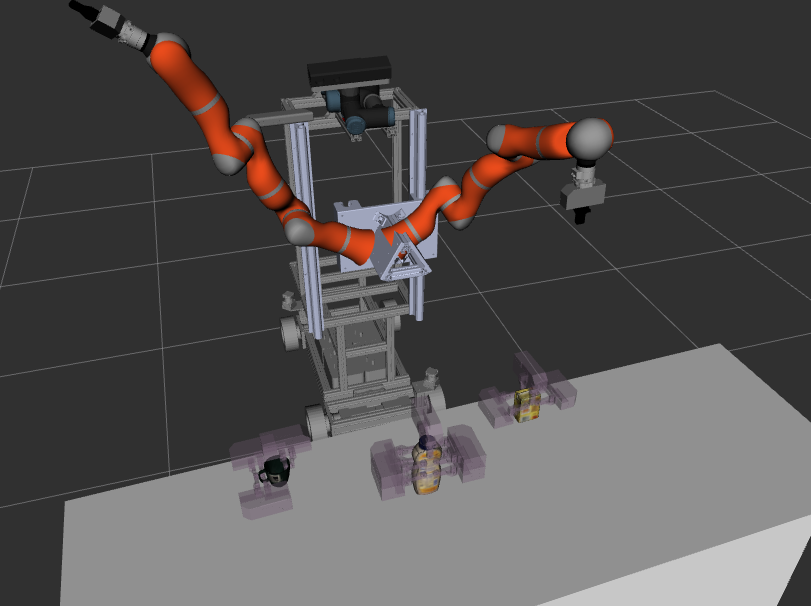
\includegraphics[width=0.5\linewidth]{boxy/environment.png}}
	\vspace{-12pt}
	\caption[Simulation Environment]{Simulation Environment}
	\vspace{-10pt}
	\label{fig:env}
\end{figure}

Nine different initial configurations for the robot were defined. For each configuration, the robot had to grasp the three objects shown in figure \ref{fig:env}.

For some of the initial configurations, he robot was positioned far away from the table, so that the objects were out of reach for it. This was done in order to test the base's movement. In other cases the robot was placed closer to the table, so that the arms and torso started moving from the beginning of the trajectory.


\subsection{Scenario 4: Testing with the robot}

The last experiment was executed on the real robot. The robot was placed in from of a table with one of the objects from the database. In this case, the trajectory evaluation included the execution time (the time the robot required to execute the given trajectory).

\section{Experimental Results}



% \todo{reaching or lifting object for a couple of seconds??}
Figures \ref{fig:weights} to \ref{fig:arm_vel} show the results obtained by one iteration of the motion controller. In this case, the right arm of the robot has to grasp a cup located on a table out of reach fo the robot.

\begin{figure}[H]
	\centering
	% This file was created by matplotlib2tikz v0.6.13.
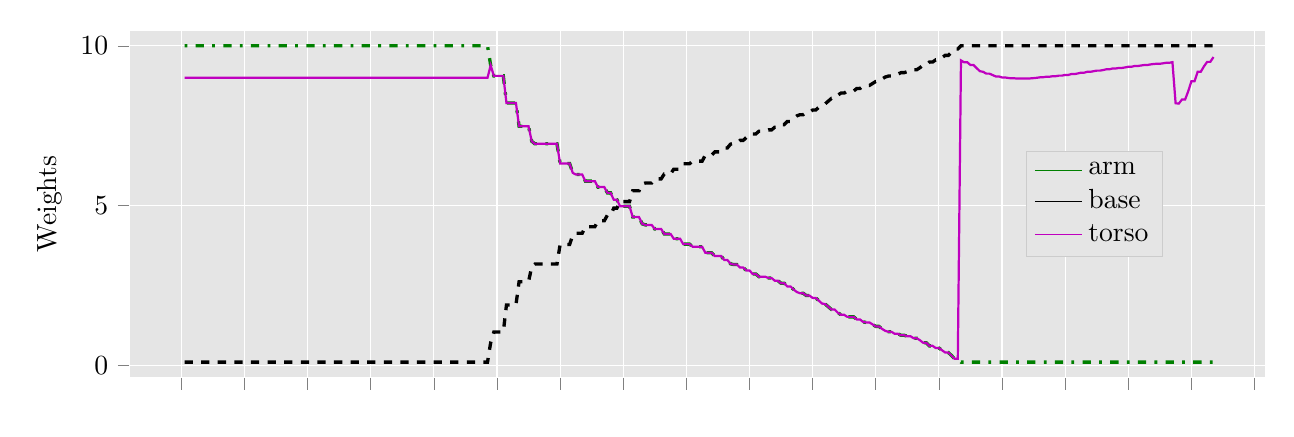
\begin{tikzpicture}

\definecolor{color0}{rgb}{0.75,0,0.75}

\begin{axis}[
%title={Arm, base and torso weights},
%xlabel={Iterations},
ylabel={Weights},
xmin=-16.35, xmax=343.35,
ymin=-0.395, ymax=10.495,
width=16cm,
height=6cm,
tick align=outside,
tick pos=left,
xmajorgrids,
x grid style={white},
ymajorgrids,
y grid style={white},
axis line style={white},
axis background/.style={fill=white!89.803921568627459!black},
legend style={at={(0.91,0.5)}, anchor=east, draw=white!80.0!black, fill=white!89.803921568627459!black},
legend entries={{arm},{base},{torso}},
legend cell align={left},
xticklabels=None
]
\addlegendimage{no markers, green!50.0!black}
\addlegendimage{no markers, black}
\addlegendimage{no markers, color0}
\addplot [very thick, green!50.0!black, dash pattern=on 1pt off 3pt on 3pt off 3pt]
table {%
1 10
2 10
3 10
4 10
5 10
6 10
7 10
8 10
9 10
10 10
11 10
12 10
13 10
14 10
15 10
16 10
17 10
18 10
19 10
20 10
21 10
22 10
23 10
24 10
25 10
26 10
27 10
28 10
29 10
30 10
31 10
32 10
33 10
34 10
35 10
36 10
37 10
38 10
39 10
40 10
41 10
42 10
43 10
44 10
45 10
46 10
47 10
48 10
49 10
50 10
51 10
52 10
53 10
54 10
55 10
56 10
57 10
58 10
59 10
60 10
61 10
62 10
63 10
64 10
65 10
66 10
67 10
68 10
69 10
70 10
71 10
72 10
73 10
74 10
75 10
76 10
77 10
78 10
79 10
80 10
81 10
82 10
83 10
84 10
85 10
86 10
87 10
88 10
89 10
90 10
91 10
92 10
93 10
94 10
95 10
96 10
97 10
98 9.38863837879147
99 9.05863837890526
100 9.05863837890526
101 9.05863837890526
102 9.05863837890526
103 8.21043380696059
104 8.21043380696059
105 8.21043380696059
106 8.21043380696059
107 7.48295987804426
108 7.48295987804426
109 7.48295987804426
110 7.48295987804426
111 7.01321231055412
112 6.93189516593896
113 6.93189516593896
114 6.93189516593896
115 6.93189516593896
116 6.93189516593896
117 6.93189516593896
118 6.93189516593896
119 6.93189516593896
120 6.31869827478432
121 6.31869827478432
122 6.31869827478432
123 6.31869827478432
124 6.02376315572432
125 5.96960045230264
126 5.96960045230264
127 5.96960045230264
128 5.76380203889371
129 5.76380203889371
130 5.76380203889371
131 5.76380203889371
132 5.57732694967849
133 5.57732694967849
134 5.57732694967849
135 5.39618792736959
136 5.39618792736959
137 5.18093155146875
138 5.18093155146875
139 4.9767700653695
140 4.9767700653695
141 4.9767700653695
142 4.9767700653695
143 4.63914692230625
144 4.63914692230625
145 4.63914692230625
146 4.42799006182836
147 4.39438637416224
148 4.39438637416224
149 4.39438637416224
150 4.26595045343693
151 4.26595045343693
152 4.26595045343693
153 4.1115817794785
154 4.1115817794785
155 4.1115817794785
156 3.96299838705074
157 3.96299838705074
158 3.96299838705074
159 3.79212275380182
160 3.79212275380182
161 3.79212275380182
162 3.71024681879868
163 3.71024681879868
164 3.71024681879868
165 3.71024681879868
166 3.52281388582086
167 3.52281388582086
168 3.52281388582086
169 3.42016931539495
170 3.42016931539495
171 3.42016931539495
172 3.29630870372592
173 3.29630870372592
174 3.17600424902726
175 3.15240694184107
176 3.15240694184107
177 3.06041992494345
178 3.06041992494345
179 2.97000285999969
180 2.97000285999969
181 2.85902780084227
182 2.85902780084227
183 2.77286925472768
184 2.77286925472768
185 2.77286925472768
186 2.73154945149062
187 2.73154945149062
188 2.64897950345558
189 2.64897950345558
190 2.5673049289761
191 2.5673049289761
192 2.46730397416921
193 2.46730397416921
194 2.36977272424109
195 2.29326725952735
196 2.25546130034102
197 2.25546130034102
198 2.18183636226213
199 2.18183636226213
200 2.10933589259532
201 2.10933589259532
202 2.02014339723245
203 1.93212967652607
204 1.91485472186242
205 1.82853575540583
206 1.74389035302755
207 1.74389035302755
208 1.64444249770138
209 1.57902959839606
210 1.57902959839606
211 1.51483478422598
212 1.51483478422598
213 1.51483478422598
214 1.43548220665633
215 1.43548220665633
216 1.3565975335528
217 1.34096713993747
218 1.34096713993747
219 1.2788219031254
220 1.21689055026798
221 1.21689055026798
222 1.13971928581219
223 1.07826859909337
224 1.0475704510928
225 1.0475704510928
226 0.986114371780824
227 0.986114371780824
228 0.939980071744355
229 0.939980071744355
230 0.909065898102437
231 0.909065898102437
232 0.846937728137582
233 0.846937728137582
234 0.784376496810485
235 0.705548721187205
236 0.705548721187205
237 0.608372686859608
238 0.608372686859608
239 0.540929829481787
240 0.540929829481787
241 0.47113987572326
242 0.399090001718742
243 0.399090001718742
244 0.304361324291846
245 0.201469157612427
246 0.201469157612427
247 0.1
248 0.1
249 0.1
250 0.1
251 0.1
252 0.1
253 0.1
254 0.1
255 0.1
256 0.1
257 0.1
258 0.1
259 0.1
260 0.1
261 0.1
262 0.1
263 0.1
264 0.1
265 0.1
266 0.1
267 0.1
268 0.1
269 0.1
270 0.1
271 0.1
272 0.1
273 0.1
274 0.1
275 0.1
276 0.1
277 0.1
278 0.1
279 0.1
280 0.1
281 0.1
282 0.1
283 0.1
284 0.1
285 0.1
286 0.1
287 0.1
288 0.1
289 0.1
290 0.1
291 0.1
292 0.1
293 0.1
294 0.1
295 0.1
296 0.1
297 0.1
298 0.1
299 0.1
300 0.1
301 0.1
302 0.1
303 0.1
304 0.1
305 0.1
306 0.1
307 0.1
308 0.1
309 0.1
310 0.1
311 0.1
312 0.1
313 0.1
314 0.1
315 0.1
316 0.1
317 0.1
318 0.1
319 0.1
320 0.1
321 0.1
322 0.1
323 0.1
324 0.1
325 0.1
326 0.1
327 0.1
};
\addplot [very thick, black, dashed]
table {%
1 0.1
2 0.1
3 0.1
4 0.1
5 0.1
6 0.1
7 0.1
8 0.1
9 0.1
10 0.1
11 0.1
12 0.1
13 0.1
14 0.1
15 0.1
16 0.1
17 0.1
18 0.1
19 0.1
20 0.1
21 0.1
22 0.1
23 0.1
24 0.1
25 0.1
26 0.1
27 0.1
28 0.1
29 0.1
30 0.1
31 0.1
32 0.1
33 0.1
34 0.1
35 0.1
36 0.1
37 0.1
38 0.1
39 0.1
40 0.1
41 0.1
42 0.1
43 0.1
44 0.1
45 0.1
46 0.1
47 0.1
48 0.1
49 0.1
50 0.1
51 0.1
52 0.1
53 0.1
54 0.1
55 0.1
56 0.1
57 0.1
58 0.1
59 0.1
60 0.1
61 0.1
62 0.1
63 0.1
64 0.1
65 0.1
66 0.1
67 0.1
68 0.1
69 0.1
70 0.1
71 0.1
72 0.1
73 0.1
74 0.1
75 0.1
76 0.1
77 0.1
78 0.1
79 0.1
80 0.1
81 0.1
82 0.1
83 0.1
84 0.1
85 0.1
86 0.1
87 0.1
88 0.1
89 0.1
90 0.1
91 0.1
92 0.1
93 0.1
94 0.1
95 0.1
96 0.1
97 0.1
98 0.711361621208532
99 1.04136162109474
100 1.04136162109474
101 1.04136162109474
102 1.04136162109474
103 1.88956619303941
104 1.88956619303941
105 1.88956619303941
106 1.88956619303941
107 2.61704012195574
108 2.61704012195574
109 2.61704012195574
110 2.61704012195574
111 3.08678768944588
112 3.16810483406104
113 3.16810483406104
114 3.16810483406104
115 3.16810483406104
116 3.16810483406104
117 3.16810483406104
118 3.16810483406104
119 3.16810483406104
120 3.78130172521568
121 3.78130172521568
122 3.78130172521568
123 3.78130172521568
124 4.07623684427568
125 4.13039954769736
126 4.13039954769736
127 4.13039954769736
128 4.33619796110629
129 4.33619796110629
130 4.33619796110629
131 4.33619796110629
132 4.52267305032151
133 4.52267305032151
134 4.52267305032151
135 4.70381207263041
136 4.70381207263041
137 4.91906844853125
138 4.91906844853125
139 5.1232299346305
140 5.1232299346305
141 5.1232299346305
142 5.1232299346305
143 5.46085307769375
144 5.46085307769375
145 5.46085307769375
146 5.67200993817164
147 5.70561362583776
148 5.70561362583776
149 5.70561362583776
150 5.83404954656307
151 5.83404954656307
152 5.83404954656307
153 5.9884182205215
154 5.9884182205215
155 5.9884182205215
156 6.13700161294926
157 6.13700161294926
158 6.13700161294926
159 6.30787724619818
160 6.30787724619818
161 6.30787724619818
162 6.38975318120132
163 6.38975318120132
164 6.38975318120132
165 6.38975318120132
166 6.57718611417914
167 6.57718611417914
168 6.57718611417914
169 6.67983068460505
170 6.67983068460505
171 6.67983068460505
172 6.80369129627408
173 6.80369129627408
174 6.92399575097274
175 6.94759305815893
176 6.94759305815893
177 7.03958007505655
178 7.03958007505655
179 7.12999714000031
180 7.12999714000031
181 7.24097219915773
182 7.24097219915773
183 7.32713074527232
184 7.32713074527232
185 7.32713074527232
186 7.36845054850938
187 7.36845054850938
188 7.45102049654442
189 7.45102049654442
190 7.5326950710239
191 7.5326950710239
192 7.63269602583079
193 7.63269602583079
194 7.7302272757589
195 7.80673274047265
196 7.84453869965898
197 7.84453869965898
198 7.91816363773787
199 7.91816363773787
200 7.99066410740468
201 7.99066410740468
202 8.07985660276755
203 8.16787032347393
204 8.18514527813758
205 8.27146424459417
206 8.35610964697245
207 8.35610964697245
208 8.45555750229862
209 8.52097040160394
210 8.52097040160394
211 8.58516521577402
212 8.58516521577402
213 8.58516521577402
214 8.66451779334367
215 8.66451779334367
216 8.7434024664472
217 8.75903286006253
218 8.75903286006253
219 8.8211780968746
220 8.88310944973202
221 8.88310944973202
222 8.96028071418781
223 9.02173140090663
224 9.0524295489072
225 9.0524295489072
226 9.11388562821918
227 9.11388562821918
228 9.16001992825564
229 9.16001992825564
230 9.19093410189756
231 9.19093410189756
232 9.25306227186242
233 9.25306227186242
234 9.31562350318952
235 9.3944512788128
236 9.3944512788128
237 9.49162731314039
238 9.49162731314039
239 9.55907017051821
240 9.55907017051821
241 9.62886012427674
242 9.70090999828126
243 9.70090999828126
244 9.79563867570815
245 9.89853084238757
246 9.89853084238757
247 10
248 10
249 10
250 10
251 10
252 10
253 10
254 10
255 10
256 10
257 10
258 10
259 10
260 10
261 10
262 10
263 10
264 10
265 10
266 10
267 10
268 10
269 10
270 10
271 10
272 10
273 10
274 10
275 10
276 10
277 10
278 10
279 10
280 10
281 10
282 10
283 10
284 10
285 10
286 10
287 10
288 10
289 10
290 10
291 10
292 10
293 10
294 10
295 10
296 10
297 10
298 10
299 10
300 10
301 10
302 10
303 10
304 10
305 10
306 10
307 10
308 10
309 10
310 10
311 10
312 10
313 10
314 10
315 10
316 10
317 10
318 10
319 10
320 10
321 10
322 10
323 10
324 10
325 10
326 10
327 10
};
\addplot [thick, color0]
table {%
1 9
2 9
3 9
4 9
5 9
6 9
7 9
8 9
9 9
10 9
11 9
12 9
13 9
14 9
15 9
16 9
17 9
18 9
19 9
20 9
21 9
22 9
23 9
24 9
25 9
26 9
27 9
28 9
29 9
30 9
31 9
32 9
33 9
34 9
35 9
36 9
37 9
38 9
39 9
40 9
41 9
42 9
43 9
44 9
45 9
46 9
47 9
48 9
49 9
50 9
51 9
52 9
53 9
54 9
55 9
56 9
57 9
58 9
59 9
60 9
61 9
62 9
63 9
64 9
65 9
66 9
67 9
68 9
69 9
70 9
71 9
72 9
73 9
74 9
75 9
76 9
77 9
78 9
79 9
80 9
81 9
82 9
83 9
84 9
85 9
86 9
87 9
88 9
89 9
90 9
91 9
92 9
93 9
94 9
95 9
96 9
97 9
98 9.38863837879147
99 9.05863837890526
100 9.05863837890526
101 9.05863837890526
102 9.05863837890526
103 8.21043380696059
104 8.21043380696059
105 8.21043380696059
106 8.21043380696059
107 7.48295987804426
108 7.48295987804426
109 7.48295987804426
110 7.48295987804426
111 7.01321231055412
112 6.93189516593896
113 6.93189516593896
114 6.93189516593896
115 6.93189516593896
116 6.93189516593896
117 6.93189516593896
118 6.93189516593896
119 6.93189516593896
120 6.31869827478432
121 6.31869827478432
122 6.31869827478432
123 6.31869827478432
124 6.02376315572432
125 5.96960045230264
126 5.96960045230264
127 5.96960045230264
128 5.76380203889371
129 5.76380203889371
130 5.76380203889371
131 5.76380203889371
132 5.57732694967849
133 5.57732694967849
134 5.57732694967849
135 5.39618792736959
136 5.39618792736959
137 5.18093155146875
138 5.18093155146875
139 4.9767700653695
140 4.9767700653695
141 4.9767700653695
142 4.9767700653695
143 4.63914692230625
144 4.63914692230625
145 4.63914692230625
146 4.42799006182836
147 4.39438637416224
148 4.39438637416224
149 4.39438637416224
150 4.26595045343693
151 4.26595045343693
152 4.26595045343693
153 4.1115817794785
154 4.1115817794785
155 4.1115817794785
156 3.96299838705074
157 3.96299838705074
158 3.96299838705074
159 3.79212275380182
160 3.79212275380182
161 3.79212275380182
162 3.71024681879868
163 3.71024681879868
164 3.71024681879868
165 3.71024681879868
166 3.52281388582086
167 3.52281388582086
168 3.52281388582086
169 3.42016931539495
170 3.42016931539495
171 3.42016931539495
172 3.29630870372592
173 3.29630870372592
174 3.17600424902726
175 3.15240694184107
176 3.15240694184107
177 3.06041992494345
178 3.06041992494345
179 2.97000285999969
180 2.97000285999969
181 2.85902780084227
182 2.85902780084227
183 2.77286925472768
184 2.77286925472768
185 2.77286925472768
186 2.73154945149062
187 2.73154945149062
188 2.64897950345558
189 2.64897950345558
190 2.5673049289761
191 2.5673049289761
192 2.46730397416921
193 2.46730397416921
194 2.36977272424109
195 2.29326725952735
196 2.25546130034102
197 2.25546130034102
198 2.18183636226213
199 2.18183636226213
200 2.10933589259532
201 2.10933589259532
202 2.02014339723245
203 1.93212967652607
204 1.91485472186242
205 1.82853575540583
206 1.74389035302755
207 1.74389035302755
208 1.64444249770138
209 1.57902959839606
210 1.57902959839606
211 1.51483478422598
212 1.51483478422598
213 1.51483478422598
214 1.43548220665633
215 1.43548220665633
216 1.3565975335528
217 1.34096713993747
218 1.34096713993747
219 1.2788219031254
220 1.21689055026798
221 1.21689055026798
222 1.13971928581219
223 1.07826859909337
224 1.0475704510928
225 1.0475704510928
226 0.986114371780824
227 0.986114371780824
228 0.939980071744355
229 0.939980071744355
230 0.909065898102437
231 0.909065898102437
232 0.846937728137582
233 0.846937728137582
234 0.784376496810485
235 0.705548721187205
236 0.705548721187205
237 0.608372686859608
238 0.608372686859608
239 0.540929829481787
240 0.540929829481787
241 0.47113987572326
242 0.399090001718742
243 0.399090001718742
244 0.304361324291846
245 0.201469157612427
246 0.201469157612427
247 9.54260532288953
248 9.48432982045021
249 9.48432982045021
250 9.39845720284583
251 9.39845720284583
252 9.29776712369568
253 9.20555816793514
254 9.18647616660771
255 9.12983293187594
256 9.12983293187594
257 9.08553997378792
258 9.04209858935045
259 9.04209858935045
260 9.00856160218338
261 9.00856160218338
262 8.99226113689884
263 8.98233948875353
264 8.98233948875353
265 8.97423711814606
266 8.97423711814606
267 8.97527018540613
268 8.97527018540613
269 8.98019434772866
270 8.98846209402964
271 8.99869394295657
272 9.01276284141611
273 9.01645532183801
274 9.03153109325244
275 9.03153109325244
276 9.04851260628507
277 9.04851260628507
278 9.06620450129553
279 9.06620450129553
280 9.08876005739871
281 9.08876005739871
282 9.1161097215032
283 9.1161097215032
284 9.13451316223714
285 9.15787012125038
286 9.15787012125038
287 9.18584900418605
288 9.18584900418605
289 9.20440191672374
290 9.22280205908315
291 9.22280205908315
292 9.2409914263658
293 9.2633444584884
294 9.2633444584884
295 9.28952654765488
296 9.28952654765488
297 9.30660294405239
298 9.30660294405239
299 9.32331847040912
300 9.34376387409266
301 9.34376387409266
302 9.36752815713424
303 9.36752815713424
304 9.38294884686004
305 9.39798017292661
306 9.39798017292661
307 9.4163130786892
308 9.43061887948637
309 9.43765855294704
310 9.43765855294704
311 9.45137688292645
312 9.4680926945907
313 9.4680926945907
314 9.48758788112076
315 8.20265855956817
316 8.19004569806326
317 8.31615443423265
318 8.31615443423265
319 8.57706696081561
320 8.88822575750952
321 8.88822575750952
322 9.19110230845573
323 9.19110230845573
324 9.358346454087
325 9.49670076476511
326 9.49670076476511
327 9.64839863976692
};
\end{axis}

\end{tikzpicture}
	\vspace{-20pt}
	\caption[Dynamic weights]{Dynamic weights of the base, torso and arm. All arm joints have the same weight. Iteration $0$ to $\approx100$: base active. Iteration $\approx100$ to $\approx250$: Whole robot active. Iteration $\approx250$ on: Arm active, torso partially active. } 
	\vspace{-15pt} \label{fig:weights}
\end{figure}
\begin{figure}[H]
	\centering
	% This file was created by matplotlib2tikz v0.6.13.
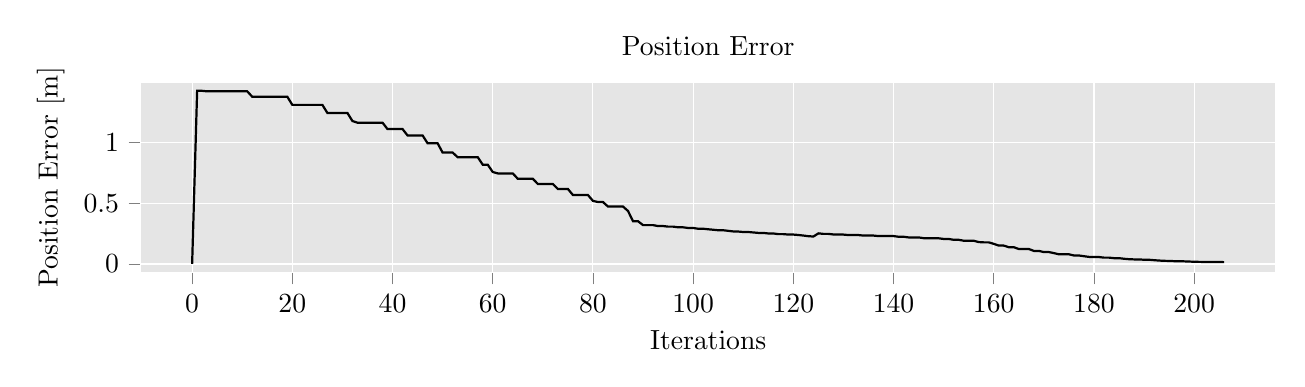
\begin{tikzpicture}

\begin{axis}[
title={Position Error},
xlabel={Iterations},
ylabel={Position Error [m]},
xmin=-10.3, xmax=216.3,
ymin=-0.0711580836737002, ymax=1.4943197571477,
width=16cm,
height=4cm,
tick align=outside,
tick pos=left,
xmajorgrids,
x grid style={white},
ymajorgrids,
y grid style={white},
axis line style={white},
axis background/.style={fill=white!89.803921568627459!black}
]
\addplot [thick, black, forget plot]
table {%
0 0
1 1.423161673474
2 1.423161673474
3 1.41910341662233
4 1.41910341662233
5 1.41910341662233
6 1.41910341662233
7 1.41910341662233
8 1.41910341662233
9 1.41910341662233
10 1.41910341662233
11 1.41910341662233
12 1.37461439918809
13 1.37461439918809
14 1.37461439918809
15 1.37461439918809
16 1.37461439918809
17 1.37461439918809
18 1.37461439918809
19 1.37461439918809
20 1.30788850795729
21 1.30788850795729
22 1.30788850795729
23 1.30788850795729
24 1.30788850795729
25 1.30788850795729
26 1.30788850795729
27 1.24105983951747
28 1.24105983951747
29 1.24105983951747
30 1.24105983951747
31 1.24105983951747
32 1.17464814493165
33 1.16142616515245
34 1.16142616515245
35 1.16142616515245
36 1.16142616515245
37 1.16142616515245
38 1.16142616515245
39 1.10876492246896
40 1.10876492246896
41 1.10876492246896
42 1.10876492246896
43 1.05650757063087
44 1.05650757063087
45 1.05650757063087
46 1.05650757063087
47 0.991851241876592
48 0.991851241876592
49 0.991851241876592
50 0.915446134221394
51 0.915446134221394
52 0.915446134221394
53 0.877825718244971
54 0.877825718244971
55 0.877825718244971
56 0.877825718244971
57 0.877825718244971
58 0.816173144458664
59 0.816173144458664
60 0.756107936270999
61 0.744506939522794
62 0.744506939522794
63 0.744506939522794
64 0.744506939522794
65 0.700200692794505
66 0.700200692794505
67 0.700200692794505
68 0.700200692794505
69 0.657696903455007
70 0.657696903455007
71 0.657696903455007
72 0.657696903455007
73 0.6166406863545
74 0.6166406863545
75 0.6166406863545
76 0.566818978752394
77 0.566818978752394
78 0.566818978752394
79 0.566818978752394
80 0.518628292113046
81 0.509146889364484
82 0.509146889364484
83 0.471878046535358
84 0.471878046535358
85 0.471878046535358
86 0.471878046535358
87 0.435528370899966
88 0.35113665140877
89 0.35113665140877
90 0.319232720891091
91 0.319232720891091
92 0.319232720891091
93 0.311571243113161
94 0.311571243113161
95 0.306867187147355
96 0.306867187147355
97 0.301208647283993
98 0.301208647283993
99 0.295769368879047
100 0.295769368879047
101 0.28941732511486
102 0.28941732511486
103 0.285262946338303
104 0.281214657903466
105 0.277179507776493
106 0.277179507776493
107 0.272251248119623
108 0.267433537341062
109 0.266472385440902
110 0.262704383110216
111 0.262704383110216
112 0.258977864031597
113 0.255280484946946
114 0.255280484946946
115 0.250699370750264
116 0.250699370750264
117 0.245252260139712
118 0.245252260139712
119 0.241641356447008
120 0.241641356447008
121 0.238045760217922
122 0.233560165895325
123 0.228190006938362
124 0.225550797833443
125 0.251572162579113
126 0.247199268587191
127 0.247199268587191
128 0.242422090477263
129 0.241437156741101
130 0.241437156741101
131 0.237421000598322
132 0.237421000598322
133 0.237421000598322
134 0.233320296684919
135 0.233320296684919
136 0.233320296684919
137 0.229115654963119
138 0.229115654963119
139 0.229115654963119
140 0.229115654963119
141 0.223682995601928
142 0.223682995601928
143 0.218126923933434
144 0.218126923933434
145 0.218126923933434
146 0.212109822811424
147 0.21087569346559
148 0.21087569346559
149 0.21087569346559
150 0.205579695968013
151 0.205579695968013
152 0.198719591502063
153 0.198719591502063
154 0.190858428278876
155 0.190858428278876
156 0.190858428278876
157 0.179980071283833
158 0.177555255587779
159 0.177555255587779
160 0.165357015435843
161 0.150890108852165
162 0.150890108852165
163 0.137522847914066
164 0.137522847914066
165 0.122838775123086
166 0.122838775123086
167 0.122838775123086
168 0.107175387884377
169 0.107175387884377
170 0.0976957733944644
171 0.0976957733944644
172 0.0891809873364261
173 0.0795168788717638
174 0.0795168788717638
175 0.0795168788717638
176 0.0696979521397309
177 0.0696979521397309
178 0.0636286062569909
179 0.0581419758815426
180 0.0567769181255327
181 0.0567769181255327
182 0.0520335569109186
183 0.0520335569109186
184 0.0476208056107397
185 0.0476208056107397
186 0.0427365445667585
187 0.0391399020712966
188 0.0374489722365945
189 0.0374489722365945
190 0.0344199933991093
191 0.0344199933991093
192 0.0310162622193478
193 0.0279606262531498
194 0.0257576470796742
195 0.0247639590531416
196 0.0229708447846483
197 0.0213943799039214
198 0.0213943799039214
199 0.0196883387217136
200 0.0182593775890196
201 0.0170537639210369
202 0.0168588038707847
203 0.0161600823520422
204 0.0161600823520422
205 0.0155706346892273
206 0.0150873969035464
};
\end{axis}

\end{tikzpicture}
	\vspace{-20pt}
	\caption[Position Error]{Position error between the EEF and the selected grasping pose} 
	\vspace{-15pt} \label{fig:error}
\end{figure}
Analyzing figures \ref{fig:weights} and \ref{fig:error} it can be seen how the weights dynamically change with the distance. During the first hundred iterations, the robot is too far away from the table, so it will move only the base. Between a certain threshold, the base's weights starts increasing and the arm's and torso's weights decrease, the robot starts to use more arm and torso and less the base. When Boxy approaches the table, the base's weight is high, so the movements are executed mainly with the arm.

\begin{figure}[H]
	\centering
	% This file was created by matplotlib2tikz v0.6.13.
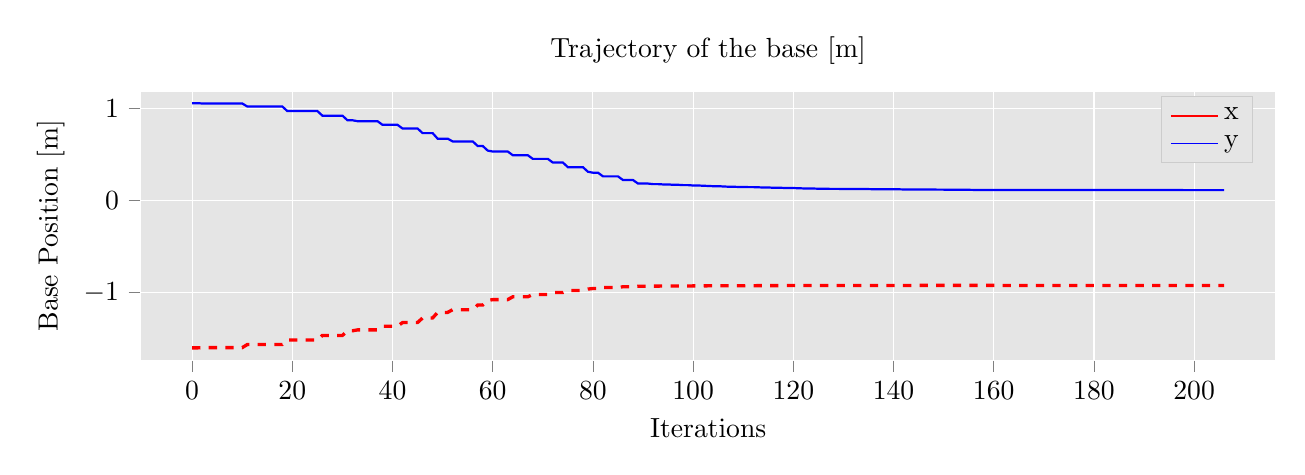
\begin{tikzpicture}

\begin{axis}[
title={Trajectory of the base [m]},
xlabel={Iterations},
ylabel={Base Position [m]},
xmin=-10.3, xmax=216.3,
ymin=-1.733, ymax=1.193,
width=16cm,
height=5cm,
tick align=outside,
tick pos=left,
xmajorgrids,
x grid style={white},
ymajorgrids,
y grid style={white},
axis line style={white},
axis background/.style={fill=white!89.803921568627459!black},
legend entries={{x},{y}},
legend cell align={left},
legend style={draw=white!80.0!black, fill=white!89.803921568627459!black}
]
\addlegendimage{no markers, red}
\addlegendimage{no markers, blue}
\addplot [very thick, red, dashed]
table {%
0 -1.6
1 -1.6
2 -1.597
3 -1.597
4 -1.597
5 -1.597
6 -1.597
7 -1.597
8 -1.597
9 -1.597
10 -1.597
11 -1.56405807907
12 -1.56405807907
13 -1.56405807907
14 -1.56405807907
15 -1.56405807907
16 -1.56405807907
17 -1.56405807907
18 -1.56405807907
19 -1.5144467024726
20 -1.5144467024726
21 -1.5144467024726
22 -1.5144467024726
23 -1.5144467024726
24 -1.5144467024726
25 -1.5144467024726
26 -1.46447406835882
27 -1.46447406835882
28 -1.46447406835882
29 -1.46447406835882
30 -1.46447406835882
31 -1.4144765073858
32 -1.4144765073858
33 -1.40447661782857
34 -1.40447661782857
35 -1.40447661782857
36 -1.40447661782857
37 -1.40447661782857
38 -1.36447675490682
39 -1.36447675490682
40 -1.36447675490682
41 -1.36447675490682
42 -1.32447679054794
43 -1.32447679054794
44 -1.32447679054794
45 -1.32447679054794
46 -1.27447680111136
47 -1.27447680111136
48 -1.27447680111136
49 -1.21447680390007
50 -1.21447680390007
51 -1.21447680390007
52 -1.18447680443961
53 -1.18447680443961
54 -1.18447680443961
55 -1.18447680443961
56 -1.18447680443961
57 -1.13447680474819
58 -1.13447680474819
59 -1.08447680480892
60 -1.07524046818883
61 -1.07524046818883
62 -1.07524046818883
63 -1.07524046818883
64 -1.04471312831992
65 -1.04471312831992
66 -1.04471312831992
67 -1.04471312831992
68 -1.01912016380541
69 -1.01912016380541
70 -1.01912016380541
71 -1.01912016380541
72 -0.997803032003999
73 -0.997803032003999
74 -0.997803032003999
75 -0.975218204865342
76 -0.975218204865342
77 -0.975218204865342
78 -0.975218204865342
79 -0.960820086794718
80 -0.95448140212623
81 -0.95448140212623
82 -0.943932479399614
83 -0.943932479399614
84 -0.943932479399614
85 -0.943932479399614
86 -0.935218731257354
87 -0.935218731257354
88 -0.935218731257354
89 -0.929284852778665
90 -0.929284852778665
91 -0.929284852778665
92 -0.928393962664367
93 -0.928393962664367
94 -0.92789253186454
95 -0.92789253186454
96 -0.927316291097345
97 -0.927316291097345
98 -0.926790137598026
99 -0.926790137598026
100 -0.92619691251295
101 -0.92619691251295
102 -0.925818433385451
103 -0.92546778223541
104 -0.925117196119697
105 -0.925117196119697
106 -0.924708749329195
107 -0.924331840806146
108 -0.924256471525831
109 -0.923981725990316
110 -0.923981725990316
111 -0.923721182188928
112 -0.923721182188928
113 -0.923471029182477
114 -0.923173563819612
115 -0.923173563819612
116 -0.922841503688237
117 -0.922841503688237
118 -0.922629596066127
119 -0.922629596066127
120 -0.922429901780819
121 -0.922198423028694
122 -0.921928330927893
123 -0.921928330927893
124 -0.921765795600105
125 -0.921583912581706
126 -0.921583912581706
127 -0.921421802577094
128 -0.921391632564588
129 -0.921391632564588
130 -0.921280607602169
131 -0.921280607602169
132 -0.921280607602169
133 -0.921179348118303
134 -0.921179348118303
135 -0.921179348118303
136 -0.921088020183272
137 -0.921088020183272
138 -0.921088020183272
139 -0.921088020183272
140 -0.92098782315279
141 -0.92098782315279
142 -0.920896038903192
143 -0.920896038903192
144 -0.920896038903192
145 -0.920828188741248
146 -0.92081601987693
147 -0.92081601987693
148 -0.92081601987693
149 -0.920779924680313
150 -0.920779924680313
151 -0.920742829785164
152 -0.920742829785164
153 -0.920729690565409
154 -0.920729690565409
155 -0.920729690565409
156 -0.920761689362019
157 -0.920771193755481
158 -0.920771193755481
159 -0.920804521650654
160 -0.920804521650654
161 -0.920833198421501
162 -0.920860653464771
163 -0.920860653464771
164 -0.920860653464771
165 -0.920891371061879
166 -0.920891371061879
167 -0.920923902603682
168 -0.920923902603682
169 -0.920943392149321
170 -0.920943392149321
171 -0.92096053619236
172 -0.92096053619236
173 -0.920979577191652
174 -0.920979577191652
175 -0.920998525549947
176 -0.920998525549947
177 -0.921010377106558
178 -0.921010377106558
179 -0.921024241612754
180 -0.921024241612754
181 -0.921034928289232
182 -0.921034928289232
183 -0.921045543618131
184 -0.921045543618131
185 -0.921059149463161
186 -0.921059149463161
187 -0.92107602181262
188 -0.92107602181262
189 -0.92108809065224
190 -0.92108809065224
191 -0.921103952717054
192 -0.92112076225457
193 -0.921134991614446
194 -0.921142511747214
195 -0.921158322304179
196 -0.921175014141524
197 -0.921175014141524
198 -0.921197055665799
199 -0.921220461611839
200 -0.921220461611839
201 -0.921250239732304
202 -0.921271735977755
203 -0.921271735977755
204 -0.921293916276054
205 -0.921293916276054
206 -0.92131691609802
};
\addplot [thick, blue]
table {%
0 1.06
1 1.06
2 1.057
3 1.057
4 1.057
5 1.057
6 1.057
7 1.057
8 1.057
9 1.057
10 1.057
11 1.02405807907
12 1.02405807907
13 1.02405807907
14 1.02405807907
15 1.02405807907
16 1.02405807907
17 1.02405807907
18 1.02405807907
19 0.974446702472604
20 0.974446702472604
21 0.974446702472604
22 0.974446702472604
23 0.974446702472604
24 0.974446702472604
25 0.974446702472604
26 0.924474068358822
27 0.924474068358822
28 0.924474068358822
29 0.924474068358822
30 0.924474068358822
31 0.874476507385801
32 0.874476507385801
33 0.864476617828568
34 0.864476617828568
35 0.864476617828568
36 0.864476617828568
37 0.864476617828568
38 0.824476754906818
39 0.824476754906818
40 0.824476754906818
41 0.824476754906818
42 0.784476790547937
43 0.784476790547937
44 0.784476790547937
45 0.784476790547937
46 0.734476801111359
47 0.734476801111359
48 0.734476801111359
49 0.674476803900066
50 0.674476803900066
51 0.674476803900066
52 0.644476804439605
53 0.644476804439605
54 0.644476804439605
55 0.644476804439605
56 0.644476804439605
57 0.594476804748189
58 0.594476804748189
59 0.544476804808915
60 0.534476804816172
61 0.534476804816172
62 0.534476804816172
63 0.534476804816172
64 0.494476804836641
65 0.494476804836641
66 0.494476804836641
67 0.494476804836641
68 0.454476804857484
69 0.454476804857484
70 0.454476804857484
71 0.454476804857484
72 0.414476804878707
73 0.414476804878707
74 0.414476804878707
75 0.364476804905702
76 0.364476804905702
77 0.364476804905702
78 0.364476804905702
79 0.314476804933276
80 0.304476804938844
81 0.304476804938844
82 0.264476804961333
83 0.264476804961333
84 0.264476804961333
85 0.264476804961333
86 0.224476804984123
87 0.224476804984123
88 0.224476804984123
89 0.186076091376362
90 0.186076091376362
91 0.186076091376362
92 0.180144792083999
93 0.180144792083999
94 0.176782658562525
95 0.176782658562525
96 0.172888030631495
97 0.172888030631495
98 0.169295215840986
99 0.169295215840986
100 0.165210350726714
101 0.165210350726714
102 0.162587334639323
103 0.160128842622251
104 0.157670209058382
105 0.157670209058382
106 0.154770852098351
107 0.152055300242471
108 0.151512161360925
109 0.149493372647414
110 0.149493372647414
111 0.147555332842583
112 0.147555332842583
113 0.145675781981009
114 0.143410690957842
115 0.143410690957842
116 0.140830220801471
117 0.140830220801471
118 0.139161694028975
119 0.139161694028975
120 0.137559121567055
121 0.135653665403669
122 0.133407502197722
123 0.133407502197722
124 0.132001695978516
125 0.130351715971188
126 0.130351715971188
127 0.128771189955413
128 0.128464747123751
129 0.128464747123751
130 0.127283583969367
131 0.127283583969367
132 0.127283583969367
133 0.12614633937926
134 0.12614633937926
135 0.12614633937926
136 0.125052376393463
137 0.125052376393463
138 0.125052376393463
139 0.125052376393463
140 0.123743992092906
141 0.123743992092906
142 0.122470318542358
143 0.122470318542358
144 0.122470318542358
145 0.121291588456311
146 0.121061295617525
147 0.121061295617525
148 0.121061295617525
149 0.12018636887809
150 0.12018636887809
151 0.119121956420319
152 0.119121956420319
153 0.1181404746572
154 0.1181404746572
155 0.1181404746572
156 0.117313694241853
157 0.11715914169192
158 0.11715914169192
159 0.116763204935963
160 0.116763204935963
161 0.116592045510715
162 0.116433945836664
163 0.116433945836664
164 0.116433945836664
165 0.116260975382485
166 0.116260975382485
167 0.116077146910816
168 0.116077146910816
169 0.115966222373377
170 0.115966222373377
171 0.115867466731942
172 0.115867466731942
173 0.115756349430836
174 0.115756349430836
175 0.115646319448912
176 0.115646319448912
177 0.115578836236855
178 0.115578836236855
179 0.115503951365173
180 0.115503951365173
181 0.115453038033154
182 0.115453038033154
183 0.115405960546106
184 0.115405960546106
185 0.115354700159115
186 0.115354700159115
187 0.115299834971672
188 0.115299834971672
189 0.115269252464994
190 0.115269252464994
191 0.115235496241995
192 0.11520560932771
193 0.115184312534541
194 0.115174886776325
195 0.115158178105164
196 0.115143686675652
197 0.115143686675652
198 0.115128066328859
199 0.115114972584817
200 0.115114972584817
201 0.115101937531827
202 0.115095571494139
203 0.115095571494139
204 0.115090080965047
205 0.115090080965047
206 0.115085504735328
};
\end{axis}

\end{tikzpicture}
	\vspace{-20pt}
	\caption[Base Trajectory]{Trajectory of the base in $x$ and $y$}
	\vspace{-15pt} \label{fig:base_pos}
\end{figure}
\begin{figure}[H]
	\centering
	% This file was created by matplotlib2tikz v0.6.13.
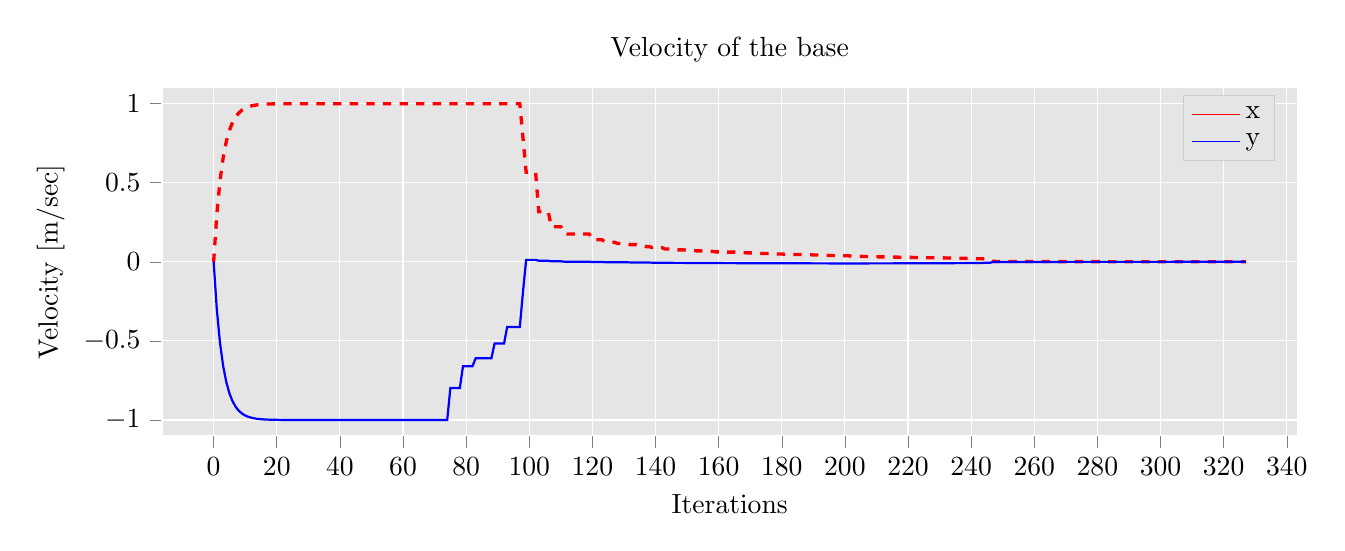
\begin{tikzpicture}

\begin{axis}[
title={Velocity of the base},
xlabel={Iterations},
ylabel={Velocity [m/sec]},
xmin=-16.35, xmax=343.35,
ymin=-1.09999999943972, ymax=1.09999999979473,
width=16cm,
height=6cm,
tick align=outside,
tick pos=left,
xmajorgrids,
x grid style={white},
ymajorgrids,
y grid style={white},
axis line style={white},
axis background/.style={fill=white!89.803921568627459!black},
legend entries={{x},{y}},
legend cell align={left},
legend style={draw=white!80.0!black, fill=white!89.803921568627459!black}
]
\addlegendimage{no markers, red}
\addlegendimage{no markers, blue}
\addplot [very thick, red, dashed]
table {%
0 0
1 0.3
2 0.51
3 0.657
4 0.7599
5 0.83193
6 0.882351
7 0.9176457
8 0.94235199
9 0.959646393
10 0.9717524751
11 0.98022673257
12 0.986158712799
13 0.9903110989593
14 0.99321776927151
15 0.995252438490057
16 0.99667670694304
17 0.997673694860128
18 0.998371586402089
19 0.998860110481463
20 0.999202077337024
21 0.999441454135916
22 0.999609017895142
23 0.999726312526599
24 0.999808418768619
25 0.999865893138033
26 0.999906125196623
27 0.999934287637636
28 0.999954001346345
29 0.999967800942442
30 0.999977460659709
31 0.999984222461796
32 0.999988955723257
33 0.99999226900628
34 0.999994588304396
35 0.999996211813077
36 0.999997348269154
37 0.999998143788408
38 0.999998700651885
39 0.99999909045632
40 0.999999363319424
41 0.999999554323597
42 0.999999688026518
43 0.999999781618562
44 0.999999847132993
45 0.999999892993095
46 0.999999925095167
47 0.999999947566617
48 0.999999963296632
49 0.999999974307642
50 0.99999998201535
51 0.999999987410745
52 0.999999991187521
53 0.999999993831265
54 0.999999995681885
55 0.99999999697732
56 0.999999997884124
57 0.999999998518887
58 0.99999999896322
59 0.999999999274254
60 0.999999999266646
61 0.999999999260229
62 0.999999999254642
63 0.99999999924963
64 0.999999999245016
65 0.999999999240674
66 0.999999999236518
67 0.999999999465562
68 0.99999999946274
69 0.999999999459975
70 0.999999999457246
71 0.999999999454539
72 0.999999999451843
73 0.999999999449151
74 0.999999999446457
75 0.99999999961252
76 0.999999999728764
77 0.999999999810135
78 0.9999999996521
79 0.99999999975647
80 0.999999999829529
81 0.999999999687637
82 0.999999999781346
83 0.999999999599348
84 0.999999999719543
85 0.99999999980368
86 0.999999999640273
87 0.999999999748191
88 0.999999999823734
89 0.999999999677018
90 0.999999999773912
91 0.999999999585727
92 0.999999999710009
93 0.999999999797006
94 0.999999999628044
95 0.99999999973963
96 0.999999999817741
97 0.999999999666038
98 0.783639946129655
99 0.566532027398449
100 0.566532027398449
101 0.566532027398449
102 0.566532027398449
103 0.317389947948394
104 0.317389947948394
105 0.317389947948394
106 0.317389947948394
107 0.221374226052071
108 0.221374226052071
109 0.221374226052071
110 0.221374226052071
111 0.181673626660572
112 0.175912401498953
113 0.175912401498953
114 0.175912401498953
115 0.175912401498953
116 0.175912401498953
117 0.175912401498953
118 0.175912401498953
119 0.175912401498953
120 0.13997696469038
121 0.13997696469038
122 0.13997696469038
123 0.13997696469038
124 0.126332160825351
125 0.124027047429103
126 0.124027047429103
127 0.124027047429103
128 0.115767134017437
129 0.115767134017437
130 0.115767134017437
131 0.115767134017437
132 0.108901187098967
133 0.108901187098967
134 0.108901187098967
135 0.102728517949029
136 0.102728517949029
137 0.0959582994296577
138 0.0959582994296577
139 0.0900406634973545
140 0.0900406634973545
141 0.0900406634973545
142 0.0900406634973545
143 0.0811879046987111
144 0.0811879046987111
145 0.0811879046987111
146 0.0761668416290684
147 0.0754008127665916
148 0.0754008127665916
149 0.0754008127665916
150 0.0725513283599198
151 0.0725513283599198
152 0.0725513283599198
153 0.0692824761291867
154 0.0692824761291867
155 0.0692824761291867
156 0.0662860010071556
157 0.0662860010071556
158 0.0662860010071556
159 0.0630084243788601
160 0.0630084243788601
161 0.0630084243788601
162 0.0614978443021977
163 0.0614978443021977
164 0.0614978443021977
165 0.0614978443021977
166 0.0581766927255096
167 0.0581766927255096
168 0.0581766927255096
169 0.056434042546078
170 0.056434042546078
171 0.056434042546078
172 0.054398571382497
173 0.054398571382497
174 0.052488672102898
175 0.0521215059508624
176 0.0521215059508624
177 0.0507125989375591
178 0.0507125989375591
179 0.0493617929091478
180 0.0493617929091478
181 0.0477481328240453
182 0.0477481328240453
183 0.0465273922943916
184 0.0465273922943916
185 0.0465273922943916
186 0.0459513272344202
187 0.0459513272344202
188 0.0448186132992693
189 0.0448186132992693
190 0.0437214926807179
191 0.0437214926807179
192 0.0424083685431964
193 0.0424083685431964
194 0.041158299040721
195 0.0401980901315713
196 0.0397300077457984
197 0.0397300077457984
198 0.0388298615718818
199 0.0388298615718818
200 0.03795827805654
201 0.03795827805654
202 0.0369054830346441
203 0.0358869440789865
204 0.0356892314169386
205 0.0347125040169577
206 0.0337713970396775
207 0.0337713970396775
208 0.0326855334070922
209 0.0319825113999489
210 0.0319825113999489
211 0.0313002609956878
212 0.0313002609956878
213 0.0313002609956878
214 0.0304672641351789
215 0.0304672641351789
216 0.0296501273297293
217 0.0294893120267265
218 0.0294893120267265
219 0.0288532199265133
220 0.028224724405256
221 0.028224724405256
222 0.0274481425038731
223 0.0268330634959774
224 0.0265277058592067
225 0.0265277058592067
226 0.0259163336749485
227 0.0259163336749485
228 0.0254581233668603
229 0.0254581233668603
230 0.0251510113004594
231 0.0251510113004594
232 0.0245328045320631
233 0.0245328045320631
234 0.0239070784954157
235 0.0231096271106575
236 0.0231098894592551
237 0.0221032312595147
238 0.0221032787502754
239 0.0213795200485544
240 0.0213795279896738
241 0.0205960072178911
242 0.0197295299133889
243 0.0197295294797202
244 0.0184398371520903
245 0.016615393425066
246 0.0166182732378135
247 0.00270373418648585
248 0.0026128516953061
249 0.00261319145881254
250 0.00249096381747509
251 0.0024913783669066
252 0.00234801175345286
253 0.00221370678674959
254 0.00218746892650675
255 0.0020913922088439
256 0.00209167405263724
257 0.0020030405131796
258 0.0019005471922461
259 0.00190087491572202
260 0.00178955193304493
261 0.00178979214441156
262 0.00172061395333867
263 0.0016561115356257
264 0.0016561115356257
265 0.00157975547523291
266 0.00157975547523291
267 0.00149612393683255
268 0.00149612393683255
269 0.0014441107068809
270 0.00139517113368503
271 0.00133530724959686
272 0.00127961516957943
273 0.00126929358171935
274 0.00122878489011091
275 0.00122878489011091
276 0.00119087253924815
277 0.00119087253924815
278 0.00115469942852002
279 0.00115469942852002
280 0.00111146846947892
281 0.00111146846947892
282 0.00106204770683439
283 0.00106204770683439
284 0.00103063919143811
285 0.000993685846203463
286 0.000993685846203463
287 0.000951624689414732
288 0.000951624689414732
289 0.000925073759110185
290 0.000899652741164823
291 0.000899652741164823
292 0.000875009247016814
293 0.000845592554315922
294 0.000845592554315922
295 0.000812099391072471
296 0.000812099391072471
297 0.000790708246148247
298 0.000790708246148247
299 0.000770129993068407
300 0.000745306403226044
301 0.000745306403226044
302 0.000716920071049524
303 0.000716920071049524
304 0.000698728672316255
305 0.000681176959522072
306 0.000681176959522072
307 0.000659944241533544
308 0.00064350308535054
309 0.000635447286604311
310 0.00063544728660431
311 0.000619843061178572
312 0.000600940690730548
313 0.000600940690730548
314 0.000579017269642604
315 0.000509624100065074
316 0.00049558542509011
317 0.000482552443330188
318 0.000482662969781215
319 0.000471129597723429
320 0.000457520274886657
321 0.000457672579783183
322 0.000442178980546268
323 0.000442273493480039
324 0.000432349893821984
325 0.000422446323223205
326 0.000422556035164441
327 0.000410456009080873
};
\addplot [thick, blue]
table {%
0 0
1 -0.3
2 -0.51
3 -0.657
4 -0.7599
5 -0.83193
6 -0.882351
7 -0.9176457
8 -0.94235199
9 -0.959646393
10 -0.9717524751
11 -0.98022673257
12 -0.986158712799
13 -0.9903110989593
14 -0.99321776927151
15 -0.995252438490057
16 -0.99667670694304
17 -0.997673694860128
18 -0.998371586402089
19 -0.998860110481463
20 -0.999202077337024
21 -0.999441454135916
22 -0.999609017895142
23 -0.999726312526599
24 -0.999808418768619
25 -0.999865893138033
26 -0.999906125196623
27 -0.999934287637636
28 -0.999954001346345
29 -0.999967800942442
30 -0.999977460659709
31 -0.999984222461796
32 -0.999988955723257
33 -0.99999226900628
34 -0.999994588304396
35 -0.999996211813077
36 -0.999997348269154
37 -0.999998143788408
38 -0.999998700651885
39 -0.99999909045632
40 -0.999999363319424
41 -0.999999554323597
42 -0.999999688026518
43 -0.999999781618562
44 -0.999999847132993
45 -0.999999892993095
46 -0.999999925095167
47 -0.999999947566617
48 -0.999999963296632
49 -0.999999974307642
50 -0.99999998201535
51 -0.999999987410745
52 -0.999999991187521
53 -0.999999993831265
54 -0.999999995681885
55 -0.99999999697732
56 -0.999999997884124
57 -0.999999998518887
58 -0.99999999896322
59 -0.999999999274254
60 -0.999999999270743
61 -0.999999999267214
62 -0.999999999263668
63 -0.999999999260105
64 -0.999999999256525
65 -0.999999999252927
66 -0.999999999249313
67 -0.999999999474519
68 -0.999999999471976
69 -0.999999999469421
70 -0.999999999466854
71 -0.999999999464274
72 -0.999999999461681
73 -0.999999999459077
74 -0.999999999456459
75 -0.797340945559786
76 -0.797340945559786
77 -0.797340945559786
78 -0.797340944565699
79 -0.660400683083055
80 -0.660400683083055
81 -0.660400682276061
82 -0.660400683083055
83 -0.610084439629956
84 -0.610084440624726
85 -0.610084440624726
86 -0.610084439731568
87 -0.610084440624726
88 -0.610084440624726
89 -0.517119191860554
90 -0.517119192602426
91 -0.517119191650865
92 -0.517119192602426
93 -0.411537232286084
94 -0.411537231510264
95 -0.411537232286084
96 -0.411537232286084
97 -0.411537231589511
98 -0.191526632023519
99 0.0124024881624943
100 0.0124024881624943
101 0.0124024881624943
102 0.0124024881624943
103 0.00696846868388927
104 0.00696846868388927
105 0.00696846868388927
106 0.00696846868388927
107 0.00317723296485743
108 0.00317723296485743
109 0.00317723296485743
110 0.00317723296485743
111 0.0011985644855719
112 0.000882617586412362
113 0.000882617586412362
114 0.000882617586412362
115 0.000882617586412362
116 0.000882617586412362
117 0.000882617586412362
118 0.000882617586412362
119 0.000882617586412362
120 -0.00133362171870529
121 -0.00133362171870529
122 -0.00133362171870529
123 -0.00133362171870529
124 -0.00227171162545019
125 -0.00244142217198885
126 -0.00244142217198885
127 -0.00244142217198885
128 -0.00307338253541629
129 -0.00307338253541629
130 -0.00307338253541629
131 -0.00307338253541629
132 -0.00363934508016761
133 -0.00363934508016761
134 -0.00363934508016761
135 -0.00415872734425366
136 -0.00415872734425366
137 -0.00474853052330384
138 -0.00474853052330384
139 -0.00528271084041008
140 -0.00528271084041008
141 -0.00528271084041008
142 -0.00528271084041008
143 -0.00612500577058505
144 -0.00612500577058505
145 -0.00612500577058505
146 -0.00661841738825295
147 -0.00669547811375535
148 -0.00669547811375535
149 -0.00669547811375535
150 -0.0069871122643946
151 -0.0069871122643946
152 -0.0069871122643946
153 -0.00732510924153017
154 -0.00732510924153017
155 -0.00732510924153017
156 -0.00763624722781373
157 -0.00763624722781373
158 -0.00763624722781373
159 -0.00797643518844516
160 -0.00797643518844516
161 -0.00797643518844516
162 -0.00813224133125335
163 -0.00813224133125335
164 -0.00813224133125335
165 -0.00813224133125335
166 -0.00847201736319667
167 -0.00847201736319667
168 -0.00847201736319667
169 -0.0086465652398124
170 -0.0086465652398124
171 -0.0086465652398124
172 -0.00884570747619642
173 -0.00884570747619642
174 -0.0090270945150602
175 -0.0090611796496956
176 -0.0090611796496956
177 -0.00918755613981152
178 -0.00918755613981152
179 -0.00930494955168437
180 -0.00930494955168437
181 -0.00943971706048759
182 -0.00943971706048759
183 -0.0095346163021729
184 -0.0095346163021729
185 -0.0095346163021729
186 -0.00957442010780587
187 -0.00957442010780587
188 -0.00965160100349236
189 -0.00965160100349236
190 -0.00972249431079492
191 -0.00972249431079492
192 -0.00979898839425124
193 -0.00979898839425124
194 -0.00986112455012278
195 -0.00990154097288149
196 -0.00991882904627977
197 -0.00991882904627977
198 -0.00994221852294362
199 -0.00994221852294362
200 -0.00995796556502722
201 -0.00995796556502722
202 -0.00996749998818697
203 -0.00996782005807284
204 -0.00996562008283191
205 -0.00995280781647833
206 -0.00992671288334127
207 -0.00992671288334127
208 -0.00987680108239984
209 -0.00983493047074385
210 -0.00983493047074385
211 -0.0097807127885026
212 -0.0097807127885026
213 -0.0097807127885026
214 -0.00970180679084313
215 -0.00970180679084313
216 -0.00961559678578287
217 -0.00959613841036219
218 -0.00959613841036219
219 -0.00951085072757459
220 -0.00942039391535103
221 -0.00942039391535103
222 -0.00929939797133168
223 -0.00918300480494877
224 -0.00913330048396027
225 -0.00913330048396027
226 -0.00900574132436763
227 -0.00900574132436763
228 -0.00890409200943938
229 -0.00890409200943938
230 -0.00883168347216253
231 -0.00883168347216253
232 -0.00867666547471614
233 -0.00867666547471614
234 -0.00850960508404988
235 -0.00828213046927822
236 -0.00828214298404749
237 -0.00796405491734177
238 -0.00796405934826382
239 -0.00771212967521402
240 -0.00771213101318247
241 -0.0074197287744733
242 -0.00707510384959336
243 -0.00707510407357682
244 -0.00652745223702742
245 -0.00569012893648063
246 -0.00569152256939877
247 -0.000845760798936455
248 -0.000815071072978418
249 -0.000815114212031483
250 -0.000770884332572933
251 -0.000770936960165422
252 -0.000717764745819927
253 -0.000667220247147147
254 -0.000657088802203472
255 -0.000621188058481532
256 -0.000621223823768217
257 -0.000588595991659046
258 -0.000551300166508761
259 -0.00055134174784568
260 -0.000512051511702784
261 -0.000512081987867655
262 -0.000487937549575723
263 -0.000465887871242421
264 -0.000465887871242421
265 -0.000439999013549848
266 -0.000439999013549848
267 -0.000412600680431617
268 -0.000412600680431617
269 -0.000395943780727363
270 -0.000380605247161267
271 -0.00036177778858177
272 -0.000344660513617211
273 -0.000341590040959094
274 -0.000329573583985747
275 -0.000329573583985747
276 -0.000318560854254632
277 -0.000318560854254632
278 -0.00030814724290593
279 -0.00030814724290593
280 -0.000295768987811481
281 -0.000295768987811481
282 -0.000281674884486475
283 -0.000281674884486475
284 -0.000272753776924886
285 -0.000262321032485371
286 -0.000262321032485371
287 -0.000250470633614992
288 -0.000250470633614992
289 -0.000243001323707816
290 -0.00023585171839442
291 -0.00023585171839442
292 -0.000228913970707091
293 -0.000220621033483091
294 -0.000220621033483091
295 -0.000211154287439181
296 -0.000211154287439181
297 -0.00020509339696243
298 -0.00020509339696243
299 -0.00019924942887892
300 -0.000192182960039976
301 -0.000192182960039976
302 -0.000184077166887975
303 -0.000184077166887975
304 -0.000178869282779291
305 -0.000173833948927119
306 -0.000173833948927119
307 -0.000167731430676629
308 -0.000162998222321414
309 -0.000160676925721183
310 -0.000160676925721183
311 -0.00015617557770454
312 -0.000150716450162917
313 -0.000150716450162917
314 -0.000144380633587161
315 -0.000144643248414209
316 -0.00014057220134483
317 -0.000134705786862809
318 -0.000134719792190783
319 -0.000127190546882885
320 -0.000118377784235629
321 -0.000118397103589255
322 -0.000110301391627472
323 -0.000110313386270827
324 -0.000106095397054944
325 -0.000102744989651354
326 -0.000102758919803648
327 -9.91533483693037e-05
};
\end{axis}

\end{tikzpicture}\vspace{-20pt}
	\caption[Base Velocity]{Velocity of the base}
	\vspace{-15pt} \label{fig:base_vel}
\end{figure}
\begin{figure}[H]
	\centering
	% This file was created by matplotlib2tikz v0.6.13.
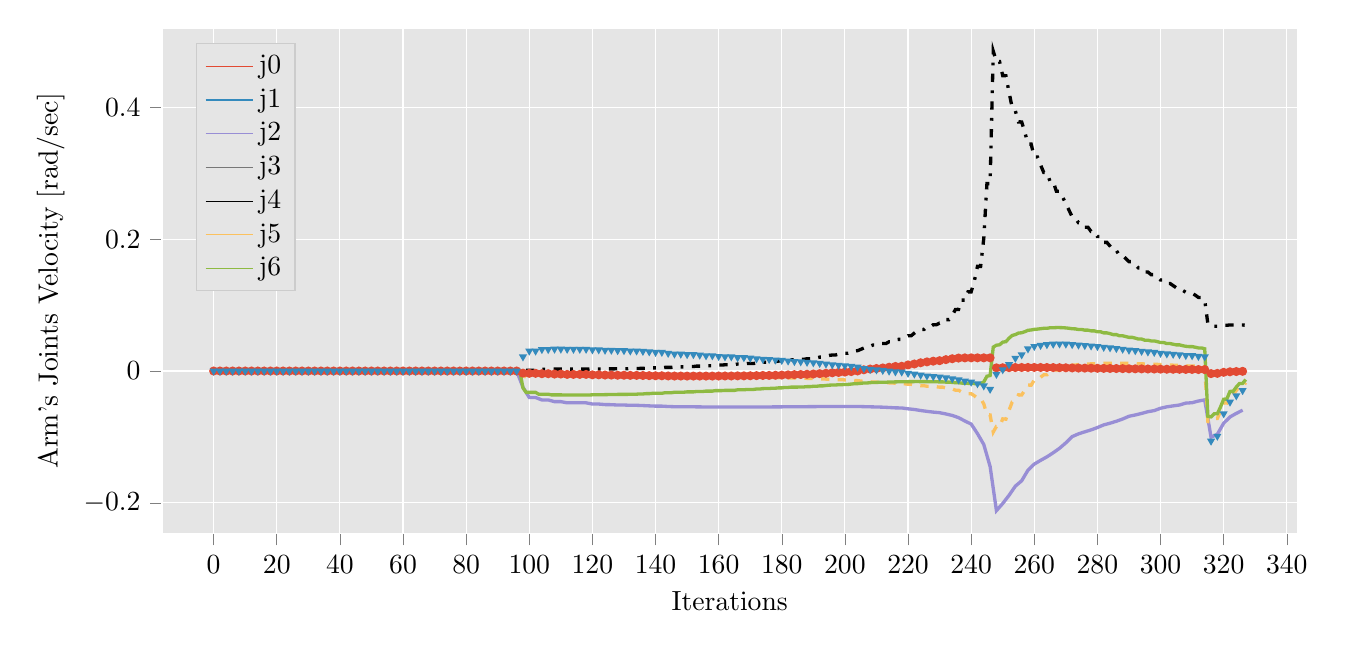
\begin{tikzpicture}

\definecolor{color1}{rgb}{0.203921568627451,0.541176470588235,0.741176470588235}
\definecolor{color0}{rgb}{0.886274509803922,0.290196078431373,0.2}
\definecolor{color3}{rgb}{0.984313725490196,0.756862745098039,0.368627450980392}
\definecolor{color2}{rgb}{0.596078431372549,0.556862745098039,0.835294117647059}
\definecolor{color4}{rgb}{0.556862745098039,0.729411764705882,0.258823529411765}

\begin{axis}[
%title={Velocity of the arm joints},
xlabel={Iterations},
ylabel={Arm's Joints Velocity [rad/sec]},
xmin=-16.35, xmax=343.35,
ymin=-0.246745048640087, ymax=0.52019802654083,
width=16cm,
height=8cm,
tick align=outside,
tick pos=left,
xmajorgrids,
x grid style={white},
ymajorgrids,
y grid style={white},
axis line style={white},
axis background/.style={fill=white!89.803921568627459!black},
legend style={at={(0.03,0.97)}, anchor=north west, draw=white!80.0!black, fill=white!89.803921568627459!black},
legend entries={{j0},{j1},{j2},{j3},{j4},{j5},{j6}},
legend cell align={left}
]
\addlegendimage{color0}
\addlegendimage{color1}
\addlegendimage{color2}
\addlegendimage{lightgray!62.222222222222221!black}
\addlegendimage{no markers, black}
\addlegendimage{no markers, color3}
\addlegendimage{no markers, color4}
\addplot [very thick, color0, mark=*, mark size=1, mark options={solid}, only marks]
table {%
0 0
2 0
4 0
6 0
8 0
10 -2.16840434497101e-19
12 0
14 0
16 0
18 0
20 0
22 0
24 0
26 0
28 0
30 0
32 0
34 0
36 0
38 0
40 0
42 0
44 0
46 -1.65436122510606e-24
48 -8.27180612553028e-25
50 0
52 0
54 1.03397576569128e-25
56 -5.16987882845642e-26
58 0
60 -7.51107895323444e-11
62 -7.58394349379613e-11
64 -7.65751338659785e-11
66 -7.73179942732516e-11
68 -5.43844838923749e-11
70 -5.49120842318597e-11
72 -5.54448001315573e-11
74 -5.59826696659815e-11
76 0
78 -7.16648307537426e-11
80 0
82 0
84 0
86 -7.41010959190436e-11
88 0
90 0
92 0
94 -7.66202134291211e-11
96 0
98 -0.00322400780800267
100 -0.00351463977466237
102 -0.00351463977466237
104 -0.00408795273877879
106 -0.00408795273877879
108 -0.00462326328190392
110 -0.00462326328190392
112 -0.00512935441466545
114 -0.00512935441466545
116 -0.00512935441466545
118 -0.00512935441466545
120 -0.00578080340234645
122 -0.00578080340234645
124 -0.0061127110361422
126 -0.00617420964566359
128 -0.00640573721725033
130 -0.00640573721725033
132 -0.00660523000755718
134 -0.00660523000755718
136 -0.00679990318433698
138 -0.00702363083511043
140 -0.00722375599316898
142 -0.00722375599316898
144 -0.00749778010909317
146 -0.00763231385829159
148 -0.00764818895731968
150 -0.00768264350859873
152 -0.00768264350859873
154 -0.00769354575199981
156 -0.00767090005179597
158 -0.00767090005179597
160 -0.00759572745412905
162 -0.00753371813039901
164 -0.00753371813039901
166 -0.00735398064133866
168 -0.00735398064133866
170 -0.00721423313763449
172 -0.00699939609088924
174 -0.00674644105385132
176 -0.00669087950054829
178 -0.0064467916407218
180 -0.00617987134758247
182 -0.00581363174784425
184 -0.00548849057816043
186 -0.0053113212641337
188 -0.00494196151341648
190 -0.00454900027511353
192 -0.0040201178051939
194 -0.00344751779009862
196 -0.0027017334320053
198 -0.00216950509802732
200 -0.00160870639708915
202 -0.000866686682613183
204 8.8200971283799e-05
206 0.00184402907771137
208 0.00299293715519379
210 0.00380683800791966
212 0.00464544717870085
214 0.0057476818580802
216 0.00693368689211808
218 0.00717699828952724
220 0.00923314520046463
222 0.0106629400056703
224 0.0125209836375003
226 0.0138544897485844
228 0.0149253916909571
230 0.0156744668593811
232 0.0172752828851833
234 0.0186376414425916
236 0.0196594103606479
238 0.019914852590162
240 0.0199787131475405
242 0.0199946782868851
244 0.0199986695717213
246 0.0199996673929303
248 0.00479891281269386
250 0.00493767514225392
252 0.00508904273038678
254 0.00526748698069397
256 0.00534015607056778
258 0.00540532043741038
260 0.0053774037730221
262 0.00533701940675983
264 0.00528165628913923
266 0.00519694806087398
268 0.00507172726417051
270 0.00488127658259802
272 0.00463214305439459
274 0.0044971539240284
276 0.00438726787278274
278 0.00427784289725453
280 0.00414275474519137
282 0.00398361283532727
284 0.00387944971297578
286 0.00375194672680894
288 0.00360289703109439
290 0.00341215182673952
292 0.00331994218030656
294 0.00320820875309198
296 0.00307917444284504
298 0.00299591623956438
300 0.00281710415055617
302 0.00270419510181723
304 0.00263146457527763
306 0.00256100842083855
308 0.00240918530833049
310 0.00237663533673238
312 0.00223688544729463
314 0.002147964749
316 -0.00396315856679872
318 -0.00359392298762987
320 -0.00197447667557736
322 -0.00120168263037246
324 -0.000800687024508574
326 -0.00048058988763846
};
\addplot [very thick, color1, mark=triangle*, mark size=0.5, mark options={solid,rotate=180}, only marks]
table {%
0 0
2 0
4 0
6 0
8 0
10 -2.16840434497101e-19
12 -2.16840434497101e-19
14 -2.16840434497101e-19
16 -5.42101086242752e-20
18 -5.42101086242752e-20
20 0
22 -1.35525271560688e-20
24 0
26 0
28 -8.470329472543e-22
30 0
32 -2.11758236813575e-22
34 -1.05879118406788e-22
36 -5.29395592033938e-23
38 -2.64697796016969e-23
40 0
42 -1.32348898008484e-23
44 -3.30872245021211e-24
46 0
48 -8.27180612553028e-25
50 -4.13590306276514e-25
52 0
54 -1.03397576569128e-25
56 0
58 -2.58493941422821e-26
60 -6.80094058851144e-11
62 -6.86691610858548e-11
64 -6.93353030013054e-11
66 -7.00079293176011e-11
68 -4.92426782086631e-11
70 -4.97203963324843e-11
72 -5.02027463412831e-11
74 -5.06897628119191e-11
76 -2.58493941422821e-26
78 -6.48892469704704e-11
80 -1.29246970711411e-26
82 -1.29246970711411e-26
84 -2.58493941422821e-26
86 -6.70951738179076e-11
88 -1.29246970711411e-26
90 -1.29246970711411e-26
92 0
94 -6.9376120516787e-11
96 0
98 0.021534016309381
100 0.0304000493863946
102 0.0304000493863946
104 0.0327286315960971
106 0.0327286315960971
108 0.0333058194574727
110 0.0333058194574727
112 0.0331111664339655
114 0.0331111664339655
116 0.0331111664339655
118 0.0331111664339655
120 0.0323007406307435
122 0.0323007406307435
124 0.0317237251925745
126 0.0315991905565265
128 0.0310792338412906
130 0.0310792338412906
132 0.0305315040312684
134 0.0305315040312684
136 0.0299547196079603
138 0.0291999952605801
140 0.0284115798409724
142 0.0284115798409724
144 0.0269325715380638
146 0.0259012234628672
148 0.0257280975509818
150 0.0250428023532234
152 0.0250428023532234
154 0.0241749909427784
156 0.0232940589340918
158 0.0232940589340918
160 0.0222240276893864
162 0.021690103321277
164 0.021690103321277
166 0.0204096712705383
168 0.0204096712705383
170 0.0196765436323388
172 0.0187616191538686
174 0.0178388411218849
176 0.0176539499105876
178 0.0169246013067787
180 0.0161862080224933
182 0.0152490633459241
184 0.0145026618048492
186 0.0141446054815337
188 0.0134088978184084
190 0.0126584852484926
192 0.0117136409552891
194 0.0107659052885359
196 0.00961739343836934
198 0.00886612831144594
200 0.00810844887995745
202 0.00714922781310602
204 0.00597177385354001
206 0.00395181234214103
208 0.00272079369268933
210 0.00187867114480305
212 0.00104031550891222
214 -3.28829249148681e-05
216 -0.00116224673667128
218 -0.00139006729723883
220 -0.00327705900835246
222 -0.00455917222107546
224 -0.00619484130337199
226 -0.00735033963830463
228 -0.00827252028223134
230 -0.00891459428331951
232 -0.010277911820768
234 -0.0116733542807976
236 -0.0133786446161374
238 -0.0153021965630678
240 -0.016602627760046
242 -0.019134421267836
244 -0.0224994221489487
246 -0.0276140737385946
248 -0.00497831012841533
250 0.00211567326196995
252 0.00979740957446604
254 0.0195613327992283
256 0.0246795520535948
258 0.0337046296104311
260 0.0374129952825002
262 0.0389663020427186
264 0.0401346833874441
266 0.040891111548443
268 0.0411987229826264
270 0.0409607694323028
272 0.0402477776775488
274 0.0395259941542096
276 0.0388418605244171
278 0.0381210959633141
280 0.0371993514541401
282 0.0360821863433725
284 0.0353307383522803
286 0.034376095896828
288 0.0332370631112269
290 0.0317429457421335
292 0.0310127102305594
294 0.0301211280589887
296 0.0290855046224879
298 0.0284148272598265
300 0.0269692383839249
302 0.0260544703184129
304 0.0254646599101058
306 0.0248927958968415
308 0.0236595954808915
310 0.0233950315334766
312 0.0222576289480482
314 0.0215328536954995
316 -0.106282705912533
318 -0.0988173060460381
320 -0.064821119265805
322 -0.0470475609562549
324 -0.0374882787360728
326 -0.0295447062099664
};
\addplot [very thick, color2]
table {%
0 0
2 0
4 0
6 0
8 0
10 0
12 0
14 -1.0842021724855e-19
16 -5.42101086242752e-20
18 -2.71050543121376e-20
20 -1.35525271560688e-20
22 -6.7762635780344e-21
24 -3.3881317890172e-21
26 -1.6940658945086e-21
28 -8.470329472543e-22
30 -4.2351647362715e-22
32 -2.11758236813575e-22
34 -1.05879118406788e-22
36 -5.29395592033938e-23
38 -2.64697796016969e-23
40 0
42 -1.32348898008484e-23
44 -6.61744490042422e-24
46 -1.65436122510606e-24
48 0
50 -4.13590306276514e-25
52 -2.06795153138257e-25
54 0
56 -5.16987882845642e-26
58 0
60 -6.84191011138258e-11
62 -6.90828307334338e-11
64 -6.97529855466807e-11
66 -7.04296638770209e-11
68 -4.95393208791129e-11
70 -5.00199167511457e-11
72 -5.05051725057695e-11
74 -5.0995122819362e-11
76 -2.58493941422821e-26
78 -6.52801460891e-11
80 -1.29246970711411e-26
82 -2.58493941422821e-26
84 -2.58493941422821e-26
86 -6.7499361785725e-11
88 -1.29246970711411e-26
90 -1.29246970711411e-26
92 -2.58493941422821e-26
94 -6.97940492292576e-11
96 -1.29246970711411e-26
98 -0.0246333107805956
100 -0.040219956338245
102 -0.040219956338245
104 -0.0438985654669562
106 -0.0438985654669562
108 -0.0464986075566804
110 -0.0464986075566804
112 -0.048298322054246
114 -0.048298322054246
116 -0.048298322054246
118 -0.048298322054246
120 -0.0501179902290826
122 -0.0501179902290826
124 -0.0509493053613041
126 -0.0510928355437419
128 -0.0516156536261824
130 -0.0516156536261824
132 -0.0520388377522807
134 -0.0520388377522807
136 -0.0524438869976749
138 -0.0528992151493051
140 -0.0533013966394165
142 -0.0533013966394165
144 -0.0538636991299207
146 -0.0541661404972186
148 -0.0542069772774045
150 -0.0543328807237161
152 -0.0543328807237161
154 -0.0544544786897914
156 -0.054543717929551
158 -0.054543717929551
160 -0.0546091218082111
162 -0.0546221204584613
164 -0.0546221204584613
166 -0.0546334835541196
168 -0.0546334835541196
170 -0.0546174450686754
172 -0.0545755775032215
174 -0.0545183777214467
176 -0.0545050739342074
178 -0.0544437381156678
180 -0.0543776811088007
182 -0.0542903587559944
184 -0.0542164228075597
186 -0.0541782620160096
188 -0.0541030222720546
190 -0.0540300309732998
192 -0.0539444538366406
194 -0.053869454270001
196 -0.0537984123211913
198 -0.0537719992136759
200 -0.0537614879568711
202 -0.0537743643825807
204 -0.0538332628932715
206 -0.0540738763791272
208 -0.0543415019461302
210 -0.0545762795609338
212 -0.0548810599775561
214 -0.0553542609636379
216 -0.055926819573993
218 -0.0560600100154173
220 -0.057360058736581
222 -0.0583873349383012
224 -0.0599454080546989
226 -0.0612540911112059
228 -0.0623811742818414
230 -0.0632266214759787
232 -0.0651675058004162
234 -0.0674198758425796
236 -0.070730316503907
238 -0.0758568548021973
240 -0.080492215199614
242 -0.0949918875494457
244 -0.11155620952525
246 -0.144840426876147
248 -0.211883999768227
250 -0.20103806968224
252 -0.188622983883601
254 -0.174734188059674
256 -0.166586661737528
258 -0.150469374819735
260 -0.141232454726358
262 -0.135573235336696
264 -0.130274436579168
266 -0.124060707838494
268 -0.11724406904045
270 -0.109001522053373
272 -0.099542508440955
274 -0.0953820262313005
276 -0.0922834465528508
278 -0.0893299416291964
280 -0.0858029710727877
282 -0.0817737477627978
284 -0.0792171399291003
286 -0.0762252033866288
288 -0.0728324509336366
290 -0.0686719931794804
292 -0.0667083179552182
294 -0.0643766996376741
296 -0.0617384318207985
298 -0.0600614094187192
300 -0.056527506843038
302 -0.0543348129406216
304 -0.0529359135524472
306 -0.0515925160711286
308 -0.0487227282299565
310 -0.0481113289452703
312 -0.0455091270893558
314 -0.0438620561697188
316 -0.10040692434457
318 -0.0960189745046938
320 -0.0791753157423931
322 -0.0697623303668309
324 -0.0642982150678771
326 -0.0594670123441806
};
\addplot [very thick, lightgray!62.222222222222221!black, mark=asterisk*, mark size=0.5, mark options={solid}, only marks]
table {%
0 0
2 -2.16840434497101e-19
4 -2.16840434497101e-19
6 -2.16840434497101e-19
8 -2.16840434497101e-19
10 -2.16840434497101e-19
12 -2.16840434497101e-19
14 -1.0842021724855e-19
16 -5.42101086242752e-20
18 0
20 0
22 -6.7762635780344e-21
24 0
26 -3.3881317890172e-21
28 -8.470329472543e-22
30 -8.470329472543e-22
32 -2.11758236813575e-22
34 -1.05879118406788e-22
36 -5.29395592033938e-23
38 -2.64697796016969e-23
40 -1.32348898008484e-23
42 0
44 0
46 -1.65436122510606e-24
48 -8.27180612553028e-25
50 -4.13590306276514e-25
52 -2.06795153138257e-25
54 -1.03397576569128e-25
56 0
58 0
60 -6.88287962830809e-11
62 -6.94965004399077e-11
64 -7.01706681506822e-11
66 -7.08513984364407e-11
68 -4.9835963432643e-11
70 -5.0319437169807e-11
72 -5.0807598728651e-11
74 -5.13004828268049e-11
76 -2.58493941422821e-26
78 -6.56710452077297e-11
80 0
82 -1.29246970711411e-26
84 -2.58493941422821e-26
86 -6.7903549536702e-11
88 0
90 -2.58493941422821e-26
92 -2.58493941422821e-26
94 -7.02119777248877e-11
96 -1.29246970711411e-26
98 0.0179877966567352
100 0.0258605587485976
102 0.0258605587485976
104 0.0276355781531231
106 0.0276355781531231
108 0.0279714700699986
110 0.0279714700699986
112 0.0276455948134402
114 0.0276455948134402
116 0.0276455948134402
118 0.0276455948134402
120 0.0267115745911585
122 0.0267115745911585
124 0.0260780306786894
126 0.0259430505317081
128 0.0253827963973299
130 0.0253827963973299
132 0.0247968276307133
134 0.0247968276307133
136 0.0241820385758819
138 0.0233800385777935
140 0.0225440666126166
142 0.0225440666126166
144 0.0209776617305886
146 0.019885863501192
148 0.0197024853990103
150 0.0189756885191669
152 0.0189756885191669
154 0.018054671398651
156 0.0171190661109786
158 0.0171190661109786
160 0.015981547243288
162 0.0154132454327099
164 0.0154132454327099
166 0.0140503670460694
168 0.0140503670460694
170 0.0132692306553403
172 0.0122935191280714
174 0.0113090781072232
176 0.0111117800729382
178 0.0103329992019922
180 0.0095447213929514
182 0.00854470698797801
184 0.00774831622067447
186 0.0073660351255728
188 0.00658127342251847
190 0.00578169697636303
192 0.0047761153958151
194 0.00376895138814065
196 0.00255092433355743
198 0.0017558823800533
200 0.000955665861654864
202 -5.48368449076662e-05
204 -0.00129102721037124
206 -0.00339984833251784
208 -0.00467690364622934
210 -0.00554712889621565
212 -0.00641049943964085
214 -0.00751219425781697
216 -0.00866791152527403
218 -0.00890065395217474
220 -0.0108251570035022
222 -0.0121304367835485
224 -0.0137973831642997
226 -0.0149807781216388
228 -0.0159279359450213
230 -0.0165905509434269
232 -0.0180065451077369
234 -0.0195132265695673
236 -0.0215067983688806
238 -0.0241406944462575
240 -0.0262328528303984
242 -0.0319218315083633
244 -0.0329610846266521
246 -0.0309938059830377
248 -0.0297343809572799
250 -0.0285450057189895
252 -0.0256957383981384
254 -0.0243996785797234
256 -0.0234134402351431
258 -0.0222131810730488
260 -0.020844382433804
262 -0.0191785722772955
264 -0.0177614365954363
266 -0.0153864499786581
268 -0.0130620287907806
270 -0.0106005857325735
272 -0.00806180275905799
274 -0.00718146039528842
276 -0.00661309526032433
278 -0.00611654069186258
280 -0.00556814737422529
282 -0.00499288860872626
284 -0.0046603568169752
286 -0.0043205306745867
288 -0.00397824892672974
290 -0.00362883624840157
292 -0.00348480985694452
294 -0.00333252274226207
296 -0.00318152198114413
298 -0.00309621914957025
300 -0.00294239842777817
302 -0.00286161597087019
304 -0.00281538205358394
306 -0.00277456218719812
308 -0.00269718503662206
310 -0.00268226065170514
312 -0.00262244786454261
314 -0.00258814468426672
316 -0.00965918884674188
318 -0.00927282129287299
320 -0.00880145287715273
322 -0.0082686520203672
324 -0.00761708224116253
326 -0.00723301989212022
};
\addplot [very thick, black, dash pattern=on 1pt off 3pt on 3pt off 3pt]
table {%
0 0
1 -2.16840434497101e-19
2 -2.16840434497101e-19
3 -2.16840434497101e-19
4 0
5 -2.16840434497101e-19
6 -2.16840434497101e-19
7 -2.16840434497101e-19
8 -2.16840434497101e-19
9 -2.16840434497101e-19
10 -2.16840434497101e-19
11 0
12 -2.16840434497101e-19
13 0
14 -1.0842021724855e-19
15 -1.0842021724855e-19
16 -1.0842021724855e-19
17 -5.42101086242752e-20
18 0
19 -2.71050543121376e-20
20 -1.35525271560688e-20
21 0
22 -6.7762635780344e-21
23 -6.7762635780344e-21
24 -6.7762635780344e-21
25 -3.3881317890172e-21
26 0
27 0
28 -8.470329472543e-22
29 0
30 -4.2351647362715e-22
31 -4.2351647362715e-22
32 -2.11758236813575e-22
33 -2.11758236813575e-22
34 0
35 0
36 0
37 0
38 0
39 0
40 -2.64697796016969e-23
41 0
42 0
43 0
44 0
45 -3.30872245021211e-24
46 -1.65436122510606e-24
47 -8.27180612553028e-25
48 -8.27180612553028e-25
49 -8.27180612553028e-25
50 -8.27180612553028e-25
51 -2.06795153138257e-25
52 -2.06795153138257e-25
53 -2.06795153138257e-25
54 -1.03397576569128e-25
55 0
56 -5.16987882845642e-26
57 -5.16987882845642e-26
58 -2.58493941422821e-26
59 0
60 -6.92384915117922e-11
61 -6.95735280031947e-11
62 -6.99101700874867e-11
63 -7.02484458120844e-11
64 -7.05883506960575e-11
65 -7.09299261128478e-11
66 -7.12731329373637e-11
67 -1.29246970711411e-26
68 -5.01326061030929e-11
69 -5.03751895715025e-11
70 -5.06189576468846e-11
71 -5.08639025825789e-11
72 -5.11100248931373e-11
73 -5.13573302951298e-11
74 -5.16058428342479e-11
75 -2.58493941422821e-26
76 0
77 -1.29246970711411e-26
78 -6.60619441095189e-11
79 0
80 -1.29246970711411e-26
81 -5.93139693177286e-11
82 -1.29246970711411e-26
83 -7.60789452269872e-11
84 0
85 -1.29246970711411e-26
86 -6.83077375045194e-11
87 0
88 0
89 -6.13303052007103e-11
90 -1.29246970711411e-26
91 -7.86652275437671e-11
92 -2.58493941422821e-26
93 -1.29246970711411e-26
94 -7.0629905786837e-11
95 -2.58493941422821e-26
96 -1.29246970711411e-26
97 -6.34152899463281e-11
98 0.00593946344707019
99 0.00122451994982646
100 0.00122451994982646
101 0.00122451994982646
102 0.00122451994982646
103 0.00263863413145511
104 0.00263863413145511
105 0.00263863413145511
106 0.00263863413145511
107 0.00283619595047067
108 0.00283619595047067
109 0.00283619595047067
110 0.00283619595047067
111 0.00288671826232692
112 0.0028981612895185
113 0.0028981612895185
114 0.0028981612895185
115 0.0028981612895185
116 0.0028981612895185
117 0.0028981612895185
118 0.0028981612895185
119 0.0028981612895185
120 0.00309422901199733
121 0.00309422901199733
122 0.00309422901199733
123 0.00309422901199733
124 0.00325606417470502
125 0.00329674396680131
126 0.00329674396680131
127 0.00329674396680131
128 0.00348228044153627
129 0.00348228044153627
130 0.00348228044153627
131 0.00348228044153627
132 0.0037105669411697
133 0.0037105669411697
134 0.0037105669411697
135 0.00396043001766251
136 0.00396043001766251
137 0.00431243517647155
138 0.00431243517647155
139 0.00471005035716715
140 0.00471005035716715
141 0.00471005035716715
142 0.00471005035716715
143 0.00555159695769631
144 0.00555159695769631
145 0.00555159695769631
146 0.00619619507967516
147 0.00631091835626467
148 0.00631091835626467
149 0.00631091835626467
150 0.00679086754347121
151 0.00679086754347121
152 0.00679086754347121
153 0.00743230044383541
154 0.00743230044383541
155 0.00743230044383541
156 0.00811946314321567
157 0.00811946314321567
158 0.00811946314321567
159 0.00900522726756366
160 0.00900522726756366
161 0.00900522726756366
162 0.0094724148669153
163 0.0094724148669153
164 0.0094724148669153
165 0.0094724148669153
166 0.0106336808950619
167 0.0106336808950619
168 0.0106336808950619
169 0.0113390816066721
170 0.0113390816066721
171 0.0113390816066721
172 0.0122637576062635
173 0.0122637576062635
174 0.0132398609429147
175 0.0134412036795725
176 0.0134412036795725
177 0.0142626171368718
178 0.0142626171368718
179 0.0151206776309627
180 0.0151206776309627
181 0.0162479531885738
182 0.0162479531885738
183 0.0171881614731713
184 0.0171881614731713
185 0.0171881614731713
186 0.0176636012078285
187 0.0176636012078285
188 0.0186530445095447
189 0.0186530445095447
190 0.0196895634717422
191 0.0196895634717422
192 0.0210467078501215
193 0.0210467078501215
194 0.0224731475501228
195 0.0236697499473334
196 0.0242880650870365
197 0.0242880650870365
198 0.025548189988616
199 0.025548189988616
200 0.0268650093549148
201 0.0268650093549148
202 0.0285985649966907
203 0.0304462941543136
204 0.0308259502862674
205 0.0328180972787845
206 0.0349354251560634
207 0.0349354251560634
208 0.0376581049564868
209 0.0396094831220242
210 0.0396094831220242
211 0.0416583824966723
212 0.0416583824966723
213 0.0416583824966723
214 0.0444056745491115
215 0.0444056745491115
216 0.047415957260574
217 0.0480472190945625
218 0.0480472190945625
219 0.0506832893194784
220 0.0535466599161064
221 0.0535466599161064
222 0.0574991851606623
223 0.0611407557538486
224 0.0628733528356912
225 0.0628733528356912
226 0.0669282450470475
227 0.0669282450470475
228 0.0702831769157963
229 0.0702831769157963
230 0.0726960904154408
231 0.0726960904154408
232 0.0780129126831747
233 0.0780129126831747
234 0.0841442024301786
235 0.0933183582018663
236 0.0933011596504226
237 0.107557801865608
238 0.107553038490597
239 0.120128477963297
240 0.120127182947843
241 0.136517910529487
242 0.158749665836963
243 0.158749462583242
244 0.201448527870457
245 0.284439863133427
246 0.284319250829047
247 0.48533697766897
248 0.469673870616681
249 0.469608548334998
250 0.448269651693403
251 0.448189982222178
252 0.423005769835335
253 0.399527871773303
254 0.394842570430907
255 0.378055051337215
256 0.378000954049661
257 0.362505328273019
258 0.344457457228178
259 0.344394580701635
260 0.324893601706198
261 0.324847522763429
262 0.312653011505821
263 0.301210468732901
264 0.301210468732901
265 0.287588018765769
266 0.287588018765769
267 0.272674812186988
268 0.272674812186988
269 0.263400883118197
270 0.254674022454257
271 0.24400523079827
272 0.2340766020685
273 0.23223432979493
274 0.225004314789363
275 0.225004314789363
276 0.218230269206666
277 0.218230269206666
278 0.211762668201298
279 0.211762668201298
280 0.204028640354555
281 0.204028640354555
282 0.195181947043169
283 0.195181947043169
284 0.18955493411147
285 0.182922797089342
286 0.182922797089342
287 0.175363808925936
288 0.175363808925936
289 0.170584206905982
290 0.166001348219879
291 0.166001348219879
292 0.161555103715835
293 0.156239250057802
294 0.156239250057802
295 0.15017566867455
296 0.15017566867455
297 0.146297428605071
298 0.146297428605071
299 0.142561165862063
300 0.138048738351241
301 0.138048738351241
302 0.132879819843708
303 0.132879819843708
304 0.129562807470169
305 0.126358169193319
306 0.126358169193319
307 0.122477330084163
308 0.119469076231318
309 0.117994193670063
310 0.117994193670063
311 0.115133746786626
312 0.111665190310868
313 0.111665190310868
314 0.107638557148928
315 0.0714819641141706
316 0.0688782103514148
317 0.0679089848374835
318 0.0678878615133716
319 0.0685366351915691
320 0.0694239648415624
321 0.0693947663781473
322 0.0699543110852451
323 0.0699361648671746
324 0.0700189082925118
325 0.0698580276446802
326 0.0698369334661162
327 0.0694411639322923
};
\addplot [very thick, color3, dashed]
table {%
0 0
1 -2.16840434497101e-19
2 -2.16840434497101e-19
3 -2.16840434497101e-19
4 -2.16840434497101e-19
5 -2.16840434497101e-19
6 -2.16840434497101e-19
7 -2.16840434497101e-19
8 0
9 -2.16840434497101e-19
10 -2.16840434497101e-19
11 0
12 -2.16840434497101e-19
13 0
14 0
15 -1.0842021724855e-19
16 0
17 -5.42101086242752e-20
18 -5.42101086242752e-20
19 0
20 0
21 0
22 0
23 0
24 0
25 -3.3881317890172e-21
26 -1.6940658945086e-21
27 0
28 0
29 -8.470329472543e-22
30 -4.2351647362715e-22
31 0
32 -2.11758236813575e-22
33 -2.11758236813575e-22
34 -1.05879118406788e-22
35 -1.05879118406788e-22
36 0
37 0
38 -2.64697796016969e-23
39 0
40 0
41 0
42 -6.61744490042422e-24
43 -6.61744490042422e-24
44 -3.30872245021211e-24
45 -1.65436122510606e-24
46 0
47 -1.65436122510606e-24
48 -8.27180612553028e-25
49 -4.13590306276514e-25
50 -4.13590306276514e-25
51 -2.06795153138257e-25
52 0
53 0
54 0
55 0
56 0
57 -2.58493941422821e-26
58 -2.58493941422821e-26
59 0
60 -6.96481867405036e-11
61 -6.99852056843867e-11
62 -7.03238397350657e-11
63 -7.0664117079e-11
64 -7.10060332414327e-11
65 -7.13496298058783e-11
66 -7.16948674382867e-11
67 0
68 -5.04292487150829e-11
69 -5.0673267608006e-11
70 -5.0918478065546e-11
71 -5.11648723678168e-11
72 -5.14124510576237e-11
73 -5.1661219805192e-11
74 -5.19112028416908e-11
75 0
76 0
77 -1.29246970711411e-26
78 -6.64528432281486e-11
79 0
80 -1.29246970711411e-26
81 -5.96649398724308e-11
82 -1.29246970711411e-26
83 -7.65291163773441e-11
84 -2.58493941422821e-26
85 0
86 -6.87119250386559e-11
87 -2.58493941422821e-26
88 -1.29246970711411e-26
89 -6.16932063161185e-11
90 -1.29246970711411e-26
91 -7.91307022077886e-11
92 -2.58493941422821e-26
93 -1.29246970711411e-26
94 -7.10478347161481e-11
95 -2.58493941422821e-26
96 -1.29246970711411e-26
97 -6.37905288487783e-11
98 -0.0112979009804797
99 -0.00537225009527556
100 -0.00537225009527556
101 -0.00537225009527556
102 -0.00537225009527556
103 -0.00629472295574515
104 -0.00629472295574515
105 -0.00629472295574515
106 -0.00629472295574515
107 -0.00640964569043344
108 -0.00640964569043344
109 -0.00640964569043344
110 -0.00640964569043344
111 -0.0063825278312068
112 -0.00637527723022886
113 -0.00637527723022886
114 -0.00637527723022886
115 -0.00637527723022886
116 -0.00637527723022886
117 -0.00637527723022886
118 -0.00637527723022886
119 -0.00637527723022886
120 -0.00634120650199228
121 -0.00634120650199228
122 -0.00634120650199228
123 -0.00634120650199228
124 -0.00633917777707658
125 -0.00634276892529474
126 -0.00634276892529474
127 -0.00634276892529474
128 -0.00636757809828965
129 -0.00636757809828965
130 -0.00636757809828965
131 -0.00636757809828965
132 -0.00641320611326029
133 -0.00641320611326029
134 -0.00641320611326029
135 -0.00646733367917357
136 -0.00646733367917357
137 -0.00655231696543369
138 -0.00655231696543369
139 -0.00665738058357699
140 -0.00665738058357699
141 -0.00665738058357699
142 -0.00665738058357699
143 -0.00690280472151286
144 -0.00690280472151286
145 -0.00690280472151286
146 -0.0071020725076888
147 -0.00713844254291143
148 -0.00713844254291143
149 -0.00713844254291143
150 -0.00729245741958563
151 -0.00729245741958563
152 -0.00729245741958563
153 -0.00750155145534477
154 -0.00750155145534477
155 -0.00750155145534477
156 -0.00772827187592164
157 -0.00772827187592164
158 -0.00772827187592164
159 -0.00802297391483901
160 -0.00802297391483901
161 -0.00802297391483901
162 -0.00817846698129121
163 -0.00817846698129121
164 -0.00817846698129121
165 -0.00817846698129121
166 -0.00856786956702341
167 -0.00856786956702341
168 -0.00856786956702341
169 -0.00880348052018742
170 -0.00880348052018742
171 -0.00880348052018742
172 -0.00911045513526194
173 -0.00911045513526194
174 -0.00943288083083597
175 -0.00949905867590091
176 -0.00949905867590091
177 -0.00976587810718744
178 -0.00976587810718744
179 -0.0100434308999532
180 -0.0100434308999532
181 -0.0104062071295902
182 -0.0104062071295902
183 -0.0107041180506829
184 -0.0107041180506829
185 -0.0107041180506829
186 -0.0108502488480537
187 -0.0108502488480537
188 -0.0111553420143981
189 -0.0111553420143981
190 -0.0114735293689245
191 -0.0114735293689245
192 -0.0118844927827465
193 -0.0118844927827465
194 -0.012308213950366
195 -0.0126580624023532
196 -0.0128370291721712
197 -0.0128370291721712
198 -0.0131917809403414
199 -0.0131917809403414
200 -0.0135568504770066
201 -0.0135568504770066
202 -0.0140297213178735
203 -0.0145271165226496
204 -0.0146270299014635
205 -0.0151519247140435
206 -0.0156966532782592
207 -0.0156966532782592
208 -0.0163777933167392
209 -0.0168579441428583
210 -0.0168579441428583
211 -0.0173482204780926
212 -0.0173482204780926
213 -0.0173482204780926
214 -0.0179957257112559
215 -0.0179957257112559
216 -0.018702564545282
217 -0.0188487633736778
218 -0.0188487633736778
219 -0.0194530331787681
220 -0.0201094343846546
221 -0.0201094343846546
222 -0.0210171423558147
223 -0.0218531668286051
224 -0.0222462920194342
225 -0.0222462920194342
226 -0.0231703209079185
227 -0.0231703209079185
228 -0.0239399240401507
229 -0.0239399240401507
230 -0.0244954349267965
231 -0.0244954349267965
232 -0.0257278636011061
233 -0.0257278636011061
234 -0.0271188943772202
235 -0.0290589185047103
236 -0.0291002499021183
237 -0.0319629394752117
238 -0.0319750774868769
239 -0.0344175052368725
240 -0.0344209313992684
241 -0.0375115623939541
242 -0.0415844334636349
243 -0.0415850053013739
244 -0.0500207694625146
245 -0.0661872069429109
246 -0.0666477871056803
247 -0.0925925173194622
248 -0.0841363450865603
249 -0.0844880327954731
250 -0.0726352406088813
251 -0.0730642399914424
252 -0.0596312329385725
253 -0.046960693403724
254 -0.0447142244277732
255 -0.0361565483996963
256 -0.0364479983223845
257 -0.0290143686038098
258 -0.0212263259169695
259 -0.0215651333245562
260 -0.0136200620164671
261 -0.0138683731877134
262 -0.00943259881767525
263 -0.00580277031561854
264 -0.00580277031561849
265 -0.00196982710185678
266 -0.00196982710185674
267 0.00166507849783218
268 0.00166507849783219
269 0.00366068950699642
270 0.00531527978771423
271 0.00727689131625748
272 0.0088102732465019
273 0.00903270782829881
274 0.00985470688644778
275 0.0098547068864478
276 0.0104449670855107
277 0.0104449670855108
278 0.0109001928128442
279 0.0109001928128442
280 0.0113289569766195
281 0.0113289569766194
282 0.0116796383431808
283 0.0116796383431808
284 0.0118160653033307
285 0.0118552037236611
286 0.0118552037236611
287 0.0117830479684959
288 0.0117830479684959
289 0.0116668468588184
290 0.0115050246950196
291 0.0115050246950196
292 0.0113124862771174
293 0.0110285809845972
294 0.0110285809845972
295 0.0106408558956719
296 0.0106408558956719
297 0.0103596655000023
298 0.0103596655000023
299 0.0100643791793205
300 0.00967974791117928
301 0.00967974791117927
302 0.0092043652196712
303 0.0092043652196712
304 0.00888073280757404
305 0.00855556258956423
306 0.00855556258956422
307 0.00814650272300228
308 0.00781840465644379
309 0.00765425575340186
310 0.00765425575340185
311 0.00733253929467329
312 0.00693342347356823
313 0.00693342347356823
314 0.00645780210571219
315 -0.0767580368703557
316 -0.0771300169070302
317 -0.0718197741445693
318 -0.0719337768022574
319 -0.0613199577506797
320 -0.0485076197077602
321 -0.0486650038700971
322 -0.0361762841591893
323 -0.0362740354317732
324 -0.029462793020356
325 -0.023727475506881
326 -0.0238410415879282
327 -0.0176253248727587
};
\addplot [very thick, color4]
table {%
0 0
1 -2.16840434497101e-19
2 -2.16840434497101e-19
3 0
4 -2.16840434497101e-19
5 -2.16840434497101e-19
6 -2.16840434497101e-19
7 0
8 0
9 -2.16840434497101e-19
10 -2.16840434497101e-19
11 0
12 0
13 0
14 -2.16840434497101e-19
15 -1.0842021724855e-19
16 -5.42101086242752e-20
17 0
18 -2.71050543121376e-20
19 -2.71050543121376e-20
20 -2.71050543121376e-20
21 0
22 -6.7762635780344e-21
23 -6.7762635780344e-21
24 -6.7762635780344e-21
25 0
26 0
27 -1.6940658945086e-21
28 -1.6940658945086e-21
29 -8.470329472543e-22
30 -4.2351647362715e-22
31 -4.2351647362715e-22
32 -2.11758236813575e-22
33 0
34 0
35 0
36 -5.29395592033938e-23
37 -5.29395592033938e-23
38 -2.64697796016969e-23
39 0
40 0
41 -1.32348898008484e-23
42 -6.61744490042422e-24
43 -6.61744490042422e-24
44 0
45 -1.65436122510606e-24
46 -1.65436122510606e-24
47 -8.27180612553028e-25
48 -8.27180612553028e-25
49 -4.13590306276514e-25
50 0
51 -4.13590306276514e-25
52 0
53 -1.03397576569128e-25
54 -1.03397576569128e-25
55 -1.03397576569128e-25
56 -5.16987882845642e-26
57 -2.58493941422821e-26
58 0
59 -1.29246970711411e-26
60 -7.00578819692149e-11
61 -7.03968833655786e-11
62 -7.07375093826447e-11
63 -7.10797884046518e-11
64 -7.1423715786808e-11
65 -7.17693334989087e-11
66 -7.21166019392097e-11
67 0
68 -5.07258913855327e-11
69 -5.09713457029436e-11
70 -5.12179985426236e-11
71 -5.14658422114585e-11
72 -5.17148772221101e-11
73 -5.19651093152541e-11
74 -5.22165628491337e-11
75 -2.58493941422821e-26
76 -2.58493941422821e-26
77 -1.29246970711411e-26
78 -6.68437423467783e-11
79 -2.58493941422821e-26
80 -1.29246970711411e-26
81 -6.00159097766118e-11
82 -1.29246970711411e-26
83 -7.69792877445413e-11
84 -2.58493941422821e-26
85 0
86 -6.91161130064732e-11
87 -2.58493941422821e-26
88 -1.29246970711411e-26
89 -6.20561072146864e-11
90 -1.29246970711411e-26
91 -7.95961766549697e-11
92 -2.58493941422821e-26
93 -1.29246970711411e-26
94 -7.14657627780974e-11
95 0
96 -1.29246970711411e-26
97 -6.41657666670264e-11
98 -0.0256441379426164
99 -0.0323811406241425
100 -0.0323811406241425
101 -0.0323811406241425
102 -0.0323811406241425
103 -0.0352393632681192
104 -0.0352393632681192
105 -0.0352393632681192
106 -0.0352393632681192
107 -0.0362096123061744
108 -0.0362096123061744
109 -0.0362096123061744
110 -0.0362096123061744
111 -0.0363885926545303
112 -0.0363898086653355
113 -0.0363898086653355
114 -0.0363898086653355
115 -0.0363898086653355
116 -0.0363898086653355
117 -0.0363898086653355
118 -0.0363898086653355
119 -0.0363898086653355
120 -0.0361125339355018
121 -0.0361125339355018
122 -0.0361125339355018
123 -0.0361125339355018
124 -0.0358342164590845
125 -0.0357686402579853
126 -0.0357686402579853
127 -0.0357686402579853
128 -0.035482828419479
129 -0.035482828419479
130 -0.035482828419479
131 -0.035482828419479
132 -0.0351618176494359
133 -0.0351618176494359
134 -0.0351618176494359
135 -0.0348182208160482
136 -0.0348182208160482
137 -0.0343580099020172
138 -0.0343580099020172
139 -0.0338672253473968
140 -0.0338672253473968
141 -0.0338672253473968
142 -0.0338672253473968
143 -0.0329186508006449
144 -0.0329186508006449
145 -0.0329186508006449
146 -0.0322463165814172
147 -0.0321318690189618
148 -0.0321318690189618
149 -0.0321318690189618
150 -0.0316716716306009
151 -0.0316716716306009
152 -0.0316716716306009
153 -0.0310837492884811
154 -0.0310837492884811
155 -0.0310837492884811
156 -0.0304830179502278
157 -0.0304830179502278
158 -0.0304830179502278
159 -0.0297484347521887
160 -0.0297484347521887
161 -0.0297484347521887
162 -0.0293789511939566
163 -0.0293789511939566
164 -0.0293789511939566
165 -0.0293789511939566
166 -0.0284956467493512
167 -0.0284956467493512
168 -0.0284956467493512
169 -0.0279879799365238
170 -0.0279879799365238
171 -0.0279879799365238
172 -0.0273526173851826
173 -0.0273526173851826
174 -0.0267130893729041
175 -0.026585084676908
176 -0.026585084676908
177 -0.0260792871599453
178 -0.0260792871599453
179 -0.0255701249978054
180 -0.0255701249978054
181 -0.0249291254570709
182 -0.0249291254570709
183 -0.024421931978889
184 -0.024421931978889
185 -0.024421931978889
186 -0.0241788921000176
187 -0.0241788921000176
188 -0.0236844441649508
189 -0.0236844441649508
190 -0.023186676560465
191 -0.023186676560465
192 -0.0225696532776698
193 -0.0225696532776698
194 -0.0219632162849231
195 -0.0214848007930717
196 -0.0212478005267985
197 -0.0212478005267985
198 -0.0207947618459231
199 -0.0207947618459231
200 -0.020350431585679
201 -0.020350431585679
202 -0.019807796453956
203 -0.0192754512334323
204 -0.0191741321545403
205 -0.0186644042592854
206 -0.0181848618336844
207 -0.0181848618336844
208 -0.0176588572199719
209 -0.0173328535411225
210 -0.0173328535411225
211 -0.0170487191053222
212 -0.0170487191053222
213 -0.0170487191053222
214 -0.0167355332758541
215 -0.0167355332758541
216 -0.0164563768437989
217 -0.0164100503580037
218 -0.0164100503580037
219 -0.0162588499679595
220 -0.0161412628746523
221 -0.0161412628746523
222 -0.0160512289440312
223 -0.0160267987169558
224 -0.0160780960038482
225 -0.0160780960038482
226 -0.016206035395624
227 -0.016206035395624
228 -0.0163583468348558
229 -0.0163583468348558
230 -0.0164963601392441
231 -0.0164963601392441
232 -0.0168674493174422
233 -0.0168674493174422
234 -0.0172893726763902
235 -0.0177257836020848
236 -0.0178064347127736
237 -0.0183338931943172
238 -0.0183571363946585
239 -0.0187393786118128
240 -0.0187458540751978
241 -0.0190850268765512
242 -0.0192713698510758
243 -0.0192724218407651
244 -0.0166002470834615
245 -0.00788071952192335
246 -0.00693109741146542
247 0.0362677012407699
248 0.0391794435580436
249 0.0397623727998226
250 0.0438106007297655
251 0.0445218428709169
252 0.0497865677751865
253 0.0539412925689869
254 0.0552644218821209
255 0.0575564793497151
256 0.0580400459152108
257 0.0596889663576932
258 0.0617148210842934
259 0.0622771074979243
260 0.0631777655899971
261 0.0635899053003481
262 0.0642136946597593
263 0.0648173744025763
264 0.0648173744025762
265 0.0656536912683623
266 0.0656536912683622
267 0.0659013328110955
268 0.0659013328110955
269 0.0657615880583354
270 0.0653842186424484
271 0.0648886129879384
272 0.0641177363223079
273 0.0639048677756432
274 0.0630246225409777
275 0.0630246225409777
276 0.0620106056992116
277 0.0620106056992116
278 0.0609391746946729
279 0.0609391746946729
280 0.0595558241685775
281 0.0595558241685775
282 0.0578567638010467
283 0.0578567638010467
284 0.0567022206348387
285 0.0552277922977182
286 0.0552277922977182
287 0.0534490695531787
288 0.0534490695531788
289 0.0522634324209035
290 0.0510833954727472
291 0.0510833954727471
292 0.0499121581778642
293 0.048467749577266
294 0.048467749577266
295 0.0467691960264378
296 0.0467691960264378
297 0.0456574130581329
298 0.0456574130581329
299 0.0445665539033422
300 0.0432283704546133
301 0.0432283704546133
302 0.0416681141470869
303 0.0416681141470869
304 0.0406527719200902
305 0.0396611978257804
306 0.0396611978257804
307 0.0384488728799583
308 0.0375006265590389
309 0.0370332630321196
310 0.0370332630321196
311 0.0361217546249242
312 0.0350087788962199
313 0.0350087788962199
314 0.0337071459530577
315 -0.0688736583343579
316 -0.0695968680087862
317 -0.0649934451634913
318 -0.0648038022694337
319 -0.0546494467378236
320 -0.042781658639297
321 -0.0425203414692366
322 -0.0309759713104668
323 -0.0308138136428696
324 -0.0242942783109939
325 -0.0190479209083132
326 -0.0188596892279102
327 -0.0129763256386548
};
\end{axis}

\end{tikzpicture}\vspace{-20pt}
	\caption[Arm Velocity]{Velocity of each one of the arm joints} \vspace{-15pt} \label{fig:arm_vel}
\end{figure}

%% This file was created by matplotlib2tikz v0.6.13.
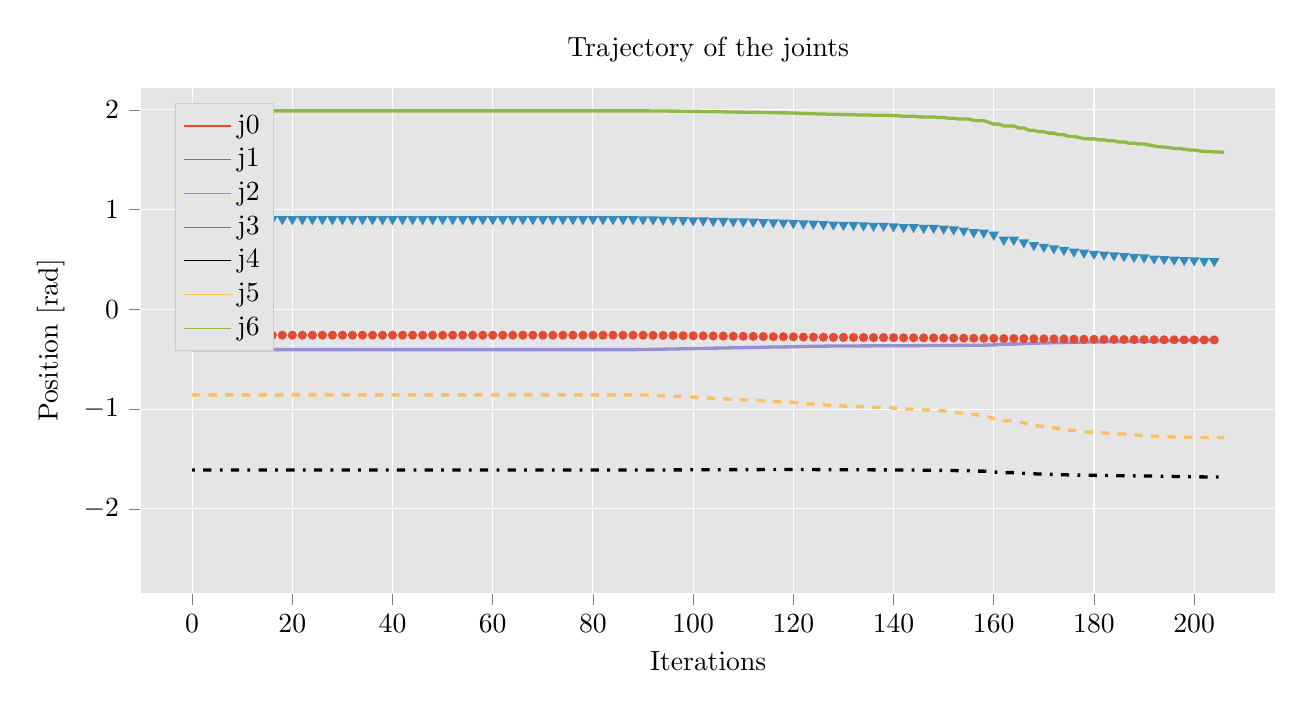
\begin{tikzpicture}

\definecolor{color1}{rgb}{0.203921568627451,0.541176470588235,0.741176470588235}
\definecolor{color0}{rgb}{0.886274509803922,0.290196078431373,0.2}
\definecolor{color3}{rgb}{0.984313725490196,0.756862745098039,0.368627450980392}
\definecolor{color2}{rgb}{0.596078431372549,0.556862745098039,0.835294117647059}
\definecolor{color4}{rgb}{0.556862745098039,0.729411764705882,0.258823529411765}

\begin{axis}[
title={Trajectory of the joints},
xlabel={Iterations},
ylabel={Position [rad]},
xmin=-10.3, xmax=216.3,
ymin=-2.84697872963385, ymax=2.22033232045874,
width=16cm,
height=8cm,
tick align=outside,
tick pos=left,
xmajorgrids,
x grid style={white},
ymajorgrids,
y grid style={white},
axis line style={white},
axis background/.style={fill=white!89.803921568627459!black},
legend style={at={(0.03,0.97)}, anchor=north west, draw=white!80.0!black, fill=white!89.803921568627459!black},
legend entries={{j0},{j1},{j2},{j3},{j4},{j5},{j6}},
legend cell align={left}
]
\addlegendimage{no markers, color0}
\addlegendimage{no markers, color1}
\addlegendimage{no markers, color2}
\addlegendimage{no markers, lightgray!62.222222222222221!black}
\addlegendimage{no markers, black}
\addlegendimage{no markers, color3}
\addlegendimage{no markers, color4}
\addplot [very thick, color0, mark=*, mark size=1, mark options={solid}, only marks]
table {%
0 -0.25941441542418
2 -0.25941441542418
4 -0.25941441542418
6 -0.25941441542418
8 -0.25941441542418
10 -0.25941441542418
12 -0.25941441542418
14 -0.25941441542418
16 -0.25941441542418
18 -0.25941441542418
20 -0.25941441542418
22 -0.25941441542418
24 -0.25941441542418
26 -0.25941441542418
28 -0.25941441542418
30 -0.25941441542418
32 -0.25941441542418
34 -0.25941441542418
36 -0.25941441542418
38 -0.25941441542418
40 -0.25941441542418
42 -0.25941441542418
44 -0.25941441542418
46 -0.25941441542418
48 -0.25941441542418
50 -0.25941441542418
52 -0.25941441542418
54 -0.25941441542418
56 -0.25941441542418
58 -0.25941441542418
60 -0.25941441542418
62 -0.25941441542418
64 -0.259414415425765
66 -0.259414415425765
68 -0.259414415427911
70 -0.259414415427911
72 -0.259414415430097
74 -0.259414415430097
76 -0.259414415432878
78 -0.259414415432878
80 -0.259414415436291
82 -0.259414415438608
84 -0.259414415438608
86 -0.259414415440955
88 -0.259414415440955
90 -0.259764415442889
92 -0.260864415443187
94 -0.261645665443243
96 -0.262638243568265
98 -0.263637071693269
100 -0.26483677872452
102 -0.265636717689364
104 -0.267236678016512
106 -0.268236671912997
108 -0.269436670196383
110 -0.270236669910281
112 -0.271036669802992
114 -0.272836669755055
116 -0.274036669755052
118 -0.274836669755052
120 -0.275636669755052
122 -0.277836669755052
124 -0.278636669755052
126 -0.279636669755052
128 -0.280836669755052
130 -0.281636669755052
132 -0.281636669755052
134 -0.282436669755051
136 -0.283236669755051
138 -0.283236669755051
140 -0.284236669755051
142 -0.285236669755051
144 -0.285236669755051
146 -0.286436669755051
148 -0.286436669755051
150 -0.287236669755051
152 -0.288236669755051
154 -0.289236669755051
156 -0.290236669755051
158 -0.290436669755051
160 -0.29123666975505
162 -0.29283666975505
164 -0.29283666975505
166 -0.29383666975505
168 -0.29503666975505
170 -0.29583666975505
172 -0.29663666975505
174 -0.29763666975505
176 -0.29883666975505
178 -0.29963666975505
180 -0.300636669755049
182 -0.301312416720959
184 -0.301932944663309
186 -0.302609243482689
188 -0.303340212510179
190 -0.303760095994043
192 -0.304676279392788
194 -0.305153259756807
196 -0.305699789400756
198 -0.306007785166708
200 -0.306294443711564
202 -0.306811527966322
204 -0.306999653671793
};
\addplot [very thick, color1, mark=triangle*, mark size=1, mark options={solid,rotate=180}, only marks]
table {%
0 0.903111279489024
2 0.903111279489024
4 0.903111279489024
6 0.903111279489024
8 0.903111279489024
10 0.903111279489024
12 0.903111279489024
14 0.903111279489024
16 0.903111279489024
18 0.903111279489024
20 0.903111279489024
22 0.903111279489024
24 0.903111279489024
26 0.903111279489024
28 0.903111279489024
30 0.903111279489024
32 0.903111279489024
34 0.903111279489024
36 0.903111279489024
38 0.903111279489024
40 0.903111279489024
42 0.903111279489024
44 0.903111279489024
46 0.903111279489024
48 0.903111279489024
50 0.903111279489024
52 0.903111279489024
54 0.903111279489024
56 0.903111279489024
58 0.903111279489024
60 0.903111279489024
62 0.903111279489024
64 0.903111279487589
66 0.903111279487589
68 0.903111279485645
70 0.903111279485645
72 0.903111279483666
74 0.903111279483666
76 0.903111279481148
78 0.903111279481148
80 0.903111279478057
82 0.90311127947596
84 0.90311127947596
86 0.903111279473835
88 0.903111279473835
90 0.902339747999252
92 0.900183064311227
94 0.898678712355856
96 0.896750239815733
98 0.894768067365157
100 0.892338158330794
102 0.890692497521502
104 0.887315959959087
106 0.885144505507628
108 0.882455086461882
110 0.880586591231657
112 0.878673060263458
114 0.874223940469755
116 0.871113158589543
118 0.868990605510906
120 0.866794925125705
122 0.860438519718078
124 0.857958097188132
126 0.854644554924972
128 0.849398259067458
130 0.845457193819289
132 0.845457193819289
134 0.841302076600103
136 0.836899555013767
138 0.836899555013767
140 0.830990865483899
142 0.824794356010544
144 0.824794356010544
146 0.816119538019976
148 0.816119538019976
150 0.809377093670721
152 0.8004507987672
154 0.789490996192099
156 0.772410755883017
158 0.768488825895009
160 0.747413468602433
162 0.697274829867068
164 0.697274829867068
166 0.671023495594617
168 0.64317392613384
170 0.626386560749523
172 0.611456707979988
174 0.594665902988233
176 0.578048218223783
178 0.567855189015558
180 0.556548598474008
182 0.548754344597335
184 0.541490908865729
186 0.533457239192405
188 0.524727858215589
190 0.519724857028592
192 0.508943990635243
194 0.503466468229148
196 0.497393055110426
198 0.49401222510908
200 0.490888527302598
202 0.485314236209367
204 0.483305563016306
};
\addplot [very thick, color2]
table {%
0 -0.403912164617797
2 -0.403912164617797
4 -0.403912164617797
6 -0.403912164617797
8 -0.403912164617797
10 -0.403912164617797
12 -0.403912164617797
14 -0.403912164617797
16 -0.403912164617797
18 -0.403912164617797
20 -0.403912164617797
22 -0.403912164617797
24 -0.403912164617797
26 -0.403912164617797
28 -0.403912164617797
30 -0.403912164617797
32 -0.403912164617797
34 -0.403912164617797
36 -0.403912164617797
38 -0.403912164617797
40 -0.403912164617797
42 -0.403912164617797
44 -0.403912164617797
46 -0.403912164617797
48 -0.403912164617797
50 -0.403912164617797
52 -0.403912164617797
54 -0.403912164617797
56 -0.403912164617797
58 -0.403912164617797
60 -0.403912164617797
62 -0.403912164617797
64 -0.403912164619241
66 -0.403912164619241
68 -0.403912164621196
70 -0.403912164621196
72 -0.403912164623188
74 -0.403912164623188
76 -0.40391216462572
78 -0.40391216462572
80 -0.40391216462883
82 -0.403912164630939
84 -0.403912164630939
86 -0.403912164633078
88 -0.403912164633078
90 -0.403020693508108
92 -0.400868095510424
94 -0.399431380182579
96 -0.397646913882095
98 -0.395876472930913
100 -0.393765031899159
102 -0.392363824813115
104 -0.389585975766994
106 -0.387865145638214
108 -0.385822261407741
110 -0.38447853716299
112 -0.383145307578491
114 -0.380175960139865
116 -0.378224517940735
118 -0.376932123730684
120 -0.375651298945512
122 -0.372176281340548
124 -0.370932589902131
126 -0.369397819959338
128 -0.368125578229006
130 -0.367391049892453
132 -0.367391049892453
134 -0.366678281402405
136 -0.365985960038486
138 -0.365985960038486
140 -0.365147585453581
142 -0.364328689427298
144 -0.364328689427298
146 -0.36338380255878
148 -0.36338380255878
150 -0.362760471327896
152 -0.361979657093843
154 -0.361126709443346
156 -0.359710387871857
158 -0.359369231895083
160 -0.356644970477499
162 -0.348788665372574
164 -0.348788665372574
166 -0.344617478468367
168 -0.340244416419112
170 -0.337643647926037
172 -0.335374362057709
174 -0.33287270062506
176 -0.330433784646622
178 -0.328928073429621
180 -0.327206322510469
182 -0.325994780285783
184 -0.324845000363633
186 -0.323483246215861
188 -0.321891618304775
190 -0.320838409858239
192 -0.318154893584577
194 -0.316453269619446
196 -0.314008394814889
198 -0.312387051791645
200 -0.310684614717644
202 -0.306993027283408
204 -0.305405206205347
};
\addplot [very thick, lightgray!62.222222222222221!black, mark=asterisk*, mark size=1, mark options={solid}, only marks]
table {%
0 -2.59999999999998
2 -2.59999999999998
4 -2.59999999999998
6 -2.59999999999998
8 -2.59999999999998
10 -2.59999999999998
12 -2.59999999999998
14 -2.59999999999998
16 -2.59999999999998
18 -2.59999999999998
20 -2.59999999999998
22 -2.59999999999998
24 -2.59999999999998
26 -2.59999999999998
28 -2.59999999999998
30 -2.59999999999998
32 -2.59999999999998
34 -2.59999999999998
36 -2.59999999999998
38 -2.59999999999998
40 -2.59999999999998
42 -2.59999999999998
44 -2.59999999999998
46 -2.59999999999998
48 -2.59999999999998
50 -2.59999999999998
52 -2.59999999999998
54 -2.59999999999998
56 -2.59999999999998
58 -2.59999999999998
60 -2.59999999999998
62 -2.59999999999998
64 -2.60000000000143
66 -2.60000000000143
68 -2.6000000000034
70 -2.6000000000034
72 -2.6000000000054
74 -2.6000000000054
76 -2.60000000000795
78 -2.60000000000795
80 -2.60000000001108
82 -2.6000000000132
84 -2.6000000000132
86 -2.60000000001535
88 -2.60000000001535
90 -2.60053981635568
92 -2.60158706005374
94 -2.60226427764515
96 -2.60307107419013
98 -2.60383335031103
100 -2.60469060473297
102 -2.60523130820747
104 -2.6062793489638
106 -2.60688055270989
108 -2.60756538833908
110 -2.60798475059018
112 -2.60838930930868
114 -2.6092500044795
116 -2.60978392440345
118 -2.61012300094539
120 -2.61044122679259
122 -2.61127303661038
124 -2.61154187026557
126 -2.61187253566144
128 -2.61224002911741
130 -2.61247076426917
132 -2.61247076426917
134 -2.612691688818
136 -2.61290598563037
138 -2.61290598563037
140 -2.61316252321648
142 -2.61341178708274
144 -2.61341178708274
146 -2.61368920517584
148 -2.61368920517584
150 -2.61386185029749
152 -2.61407363103577
154 -2.61427599680563
156 -2.61446391452255
158 -2.61450109333439
160 -2.61478171551885
162 -2.61491158489814
164 -2.61491158489814
166 -2.61506829694032
168 -2.61524539892372
170 -2.61535533808638
172 -2.61546197907415
174 -2.6155907068397
176 -2.61573747166403
178 -2.61582772791706
180 -2.61593784054577
182 -2.61602051527356
184 -2.61610110327677
186 -2.61619735377249
188 -2.61630707023546
190 -2.6163767368749
192 -2.61653805257395
194 -2.61662559561832
196 -2.61664640917509
198 -2.61650863450815
200 -2.61626015644199
202 -2.6154774819227
204 -2.61507226428469
};
\addplot [very thick, black, dash pattern=on 1pt off 3pt on 3pt off 3pt]
table {%
0 -1.61171202855818
1 -1.61171202855818
2 -1.61171202855818
3 -1.61171202855818
4 -1.61171202855818
5 -1.61171202855818
6 -1.61171202855818
7 -1.61171202855818
8 -1.61171202855818
9 -1.61171202855818
10 -1.61171202855818
11 -1.61171202855818
12 -1.61171202855818
13 -1.61171202855818
14 -1.61171202855818
15 -1.61171202855818
16 -1.61171202855818
17 -1.61171202855818
18 -1.61171202855818
19 -1.61171202855818
20 -1.61171202855818
21 -1.61171202855818
22 -1.61171202855818
23 -1.61171202855818
24 -1.61171202855818
25 -1.61171202855818
26 -1.61171202855818
27 -1.61171202855818
28 -1.61171202855818
29 -1.61171202855818
30 -1.61171202855818
31 -1.61171202855818
32 -1.61171202855818
33 -1.61171202855818
34 -1.61171202855818
35 -1.61171202855818
36 -1.61171202855818
37 -1.61171202855818
38 -1.61171202855818
39 -1.61171202855818
40 -1.61171202855818
41 -1.61171202855818
42 -1.61171202855818
43 -1.61171202855818
44 -1.61171202855818
45 -1.61171202855818
46 -1.61171202855818
47 -1.61171202855818
48 -1.61171202855818
49 -1.61171202855818
50 -1.61171202855818
51 -1.61171202855818
52 -1.61171202855818
53 -1.61171202855818
54 -1.61171202855818
55 -1.61171202855818
56 -1.61171202855818
57 -1.61171202855818
58 -1.61171202855818
59 -1.61171202855818
60 -1.61171202855818
61 -1.61171202855818
62 -1.61171202855818
63 -1.61171202855818
64 -1.61171202855964
65 -1.61171202855964
66 -1.61171202855964
67 -1.61171202855964
68 -1.61171202856162
69 -1.61171202856162
70 -1.61171202856162
71 -1.61171202856162
72 -1.61171202856363
73 -1.61171202856363
74 -1.61171202856363
75 -1.6117120285662
76 -1.6117120285662
77 -1.6117120285662
78 -1.6117120285662
79 -1.61171202856881
80 -1.61171202856934
81 -1.61171202856934
82 -1.61171202857148
83 -1.61171202857148
84 -1.61171202857148
85 -1.61171202857148
86 -1.61171202857364
87 -1.61171202857364
88 -1.61171202857364
89 -1.61142014554738
90 -1.61142014554738
91 -1.61142014554738
92 -1.61077188957171
93 -1.61077188957171
94 -1.61036405391641
95 -1.61036405391641
96 -1.6098862626115
97 -1.6098862626115
98 -1.60944516002298
99 -1.60944516002298
100 -1.608948711824
101 -1.608948711824
102 -1.60863364042272
103 -1.60834798833897
104 -1.60806249005354
105 -1.60806249005354
106 -1.60774201910644
107 -1.60746482305261
108 -1.60740942127585
109 -1.60723063665157
110 -1.60723063665157
111 -1.60707688058394
112 -1.60707688058394
113 -1.60694248158594
114 -1.60680550060305
115 -1.60680550060305
116 -1.60669545406905
117 -1.60669545406905
118 -1.60664423205443
119 -1.60664423205443
120 -1.60662431034038
121 -1.60664902057552
122 -1.60670184468838
123 -1.60670184468838
124 -1.60679221543675
125 -1.60697878447101
126 -1.60697878447101
127 -1.60754085847065
128 -1.60768003807477
129 -1.60768003807477
130 -1.60829259601352
131 -1.60829259601352
132 -1.60829259601352
133 -1.60896404300283
134 -1.60896404300283
135 -1.60896404300283
136 -1.60969992981282
137 -1.60969992981282
138 -1.60969992981282
139 -1.60969992981282
140 -1.61071969538699
141 -1.61071969538699
142 -1.61180364864213
143 -1.61180364864213
144 -1.61180364864213
145 -1.61310832113021
146 -1.61338332594686
147 -1.61338332594686
148 -1.61338332594686
149 -1.61463403948043
150 -1.61463403948043
151 -1.61629780294747
152 -1.61629780294747
153 -1.61835389878569
154 -1.61835389878569
155 -1.61835389878569
156 -1.62160246631291
157 -1.62235187193902
158 -1.62235187193902
159 -1.62661335972374
160 -1.63208822472352
161 -1.63208822472352
162 -1.63717898276602
163 -1.63717898276602
164 -1.63717898276602
165 -1.64270661308003
166 -1.64270661308003
167 -1.64845633767351
168 -1.64845633767351
169 -1.65184582712117
170 -1.65184582712117
171 -1.65476328390603
172 -1.65476328390603
173 -1.65792585983324
174 -1.65792585983324
175 -1.66083558246949
176 -1.66083558246949
177 -1.66256459525281
178 -1.6636685527042
179 -1.66440455891251
180 -1.66440455891251
181 -1.66564535181993
182 -1.66564535181993
183 -1.66679508882297
184 -1.66679508882297
185 -1.66808574401976
186 -1.66808574401976
187 -1.66952408945265
188 -1.66952408945265
189 -1.67040778059808
190 -1.67040778059808
191 -1.67146867982831
192 -1.67251313901868
193 -1.67334874152459
194 -1.67376968876399
195 -1.67462267764813
196 -1.67549687763567
197 -1.67549687763567
198 -1.67663099185739
199 -1.67782122517808
200 -1.67782122517808
201 -1.67932970222671
202 -1.68042027767367
203 -1.68042027767367
204 -1.68154855581516
205 -1.68154855581516
206 -1.68272563117356
};
\addplot [very thick, color3, dashed]
table {%
0 -0.858067121294313
1 -0.858067121294313
2 -0.858067121294313
3 -0.858067121294313
4 -0.858067121294313
5 -0.858067121294313
6 -0.858067121294313
7 -0.858067121294313
8 -0.858067121294313
9 -0.858067121294313
10 -0.858067121294313
11 -0.858067121294313
12 -0.858067121294313
13 -0.858067121294313
14 -0.858067121294313
15 -0.858067121294313
16 -0.858067121294313
17 -0.858067121294313
18 -0.858067121294313
19 -0.858067121294313
20 -0.858067121294313
21 -0.858067121294313
22 -0.858067121294313
23 -0.858067121294313
24 -0.858067121294313
25 -0.858067121294313
26 -0.858067121294313
27 -0.858067121294313
28 -0.858067121294313
29 -0.858067121294313
30 -0.858067121294313
31 -0.858067121294313
32 -0.858067121294313
33 -0.858067121294313
34 -0.858067121294313
35 -0.858067121294313
36 -0.858067121294313
37 -0.858067121294313
38 -0.858067121294313
39 -0.858067121294313
40 -0.858067121294313
41 -0.858067121294313
42 -0.858067121294313
43 -0.858067121294313
44 -0.858067121294313
45 -0.858067121294313
46 -0.858067121294313
47 -0.858067121294313
48 -0.858067121294313
49 -0.858067121294313
50 -0.858067121294313
51 -0.858067121294313
52 -0.858067121294313
53 -0.858067121294313
54 -0.858067121294313
55 -0.858067121294313
56 -0.858067121294313
57 -0.858067121294313
58 -0.858067121294313
59 -0.858067121294313
60 -0.858067121294313
61 -0.858067121294313
62 -0.858067121294313
63 -0.858067121294313
64 -0.858067121295782
65 -0.858067121295782
66 -0.858067121295782
67 -0.858067121295782
68 -0.858067121297773
69 -0.858067121297773
70 -0.858067121297773
71 -0.858067121297773
72 -0.8580671212998
73 -0.8580671212998
74 -0.8580671212998
75 -0.858067121302378
76 -0.858067121302378
77 -0.858067121302378
78 -0.858067121302378
79 -0.858067121305012
80 -0.858067121305543
81 -0.858067121305543
82 -0.858067121307691
83 -0.858067121307691
84 -0.858067121307691
85 -0.858067121307691
86 -0.858067121309868
87 -0.858067121309868
88 -0.858067121309868
89 -0.85974854513043
90 -0.85974854513043
91 -0.85974854513043
92 -0.864393842858104
93 -0.864393842858104
94 -0.867621523305136
95 -0.867621523305136
96 -0.871752595334845
97 -0.871752595334845
98 -0.875988727151836
99 -0.875988727151836
100 -0.881162737515806
101 -0.881162737515806
102 -0.884655323624869
103 -0.888228448501499
104 -0.891801653707385
105 -0.891801653707385
106 -0.896367027560062
107 -0.90105091518747
108 -0.901987713738103
109 -0.905853122076128
110 -0.905853122076128
111 -0.909788217766841
112 -0.909788217766841
113 -0.913777640872592
114 -0.918852376572595
115 -0.918852376572595
116 -0.925099340868421
117 -0.925099340868421
118 -0.929328802050579
119 -0.929328802050579
120 -0.93365238885418
121 -0.939209639678957
122 -0.945951009629409
123 -0.945951009629409
124 -0.950623379527155
125 -0.956709205707632
126 -0.956709205707632
127 -0.963353790878894
128 -0.964734586452741
129 -0.964734586452741
130 -0.970441639007592
131 -0.970441639007592
132 -0.970441639007592
133 -0.976348658241484
134 -0.976348658241484
135 -0.976348658241484
136 -0.982481864088837
137 -0.982481864088837
138 -0.982481864088837
139 -0.982481864088837
140 -0.990507836633584
141 -0.990507836633584
142 -0.998765308791343
143 -0.998765308791343
144 -0.998765308791343
145 -1.00785449998352
146 -1.0097255569475
147 -1.0097255569475
148 -1.0097255569475
149 -1.01779071521838
150 -1.01779071521838
151 -1.02825919201043
152 -1.02825919201043
153 -1.04022704938484
154 -1.04022704938484
155 -1.04022704938484
156 -1.05636823080513
157 -1.05993229248243
158 -1.05993229248243
159 -1.07734363284417
160 -1.09761217755896
161 -1.09761217755896
162 -1.11638895511031
163 -1.11638895511031
164 -1.11638895511031
165 -1.13710379714265
166 -1.13710379714265
167 -1.15933918446075
168 -1.15933918446075
169 -1.17287520281581
170 -1.17287520281581
171 -1.18506053153537
172 -1.18506053153537
173 -1.1989178918233
174 -1.1989178918233
175 -1.21288690076716
176 -1.21288690076716
177 -1.22151255491
178 -1.22923066061896
179 -1.23116024370007
180 -1.23116024370007
181 -1.23783689384613
182 -1.23783689384613
183 -1.24406291224503
184 -1.24406291224503
185 -1.25091974798971
186 -1.25091974798971
187 -1.25831917826997
188 -1.25831917826997
189 -1.26248227083416
190 -1.26248227083416
191 -1.267100666655
192 -1.27119390805955
193 -1.27410437963074
194 -1.27538650511054
195 -1.27764400558562
196 -1.27958087871826
197 -1.27958087871826
198 -1.28163021150942
199 -1.28329036954808
200 -1.28329036954808
201 -1.28485163134164
202 -1.28550439426374
203 -1.28550439426374
204 -1.2860054754043
205 -1.2860054754043
206 -1.28633808108334
};
\addplot [very thick, color4]
table {%
0 1.98999999999999
1 1.98999999999999
2 1.98999999999999
3 1.98999999999999
4 1.98999999999999
5 1.98999999999999
6 1.98999999999999
7 1.98999999999999
8 1.98999999999999
9 1.98999999999999
10 1.98999999999999
11 1.98999999999999
12 1.98999999999999
13 1.98999999999999
14 1.98999999999999
15 1.98999999999999
16 1.98999999999999
17 1.98999999999999
18 1.98999999999999
19 1.98999999999999
20 1.98999999999999
21 1.98999999999999
22 1.98999999999999
23 1.98999999999999
24 1.98999999999999
25 1.98999999999999
26 1.98999999999999
27 1.98999999999999
28 1.98999999999999
29 1.98999999999999
30 1.98999999999999
31 1.98999999999999
32 1.98999999999999
33 1.98999999999999
34 1.98999999999999
35 1.98999999999999
36 1.98999999999999
37 1.98999999999999
38 1.98999999999999
39 1.98999999999999
40 1.98999999999999
41 1.98999999999999
42 1.98999999999999
43 1.98999999999999
44 1.98999999999999
45 1.98999999999999
46 1.98999999999999
47 1.98999999999999
48 1.98999999999999
49 1.98999999999999
50 1.98999999999999
51 1.98999999999999
52 1.98999999999999
53 1.98999999999999
54 1.98999999999999
55 1.98999999999999
56 1.98999999999999
57 1.98999999999999
58 1.98999999999999
59 1.98999999999999
60 1.98999999999999
61 1.98999999999999
62 1.98999999999999
63 1.98999999999999
64 1.98999999999851
65 1.98999999999851
66 1.98999999999851
67 1.98999999999851
68 1.98999999999651
69 1.98999999999651
70 1.98999999999651
71 1.98999999999651
72 1.98999999999447
73 1.98999999999447
74 1.98999999999447
75 1.98999999999188
76 1.98999999999188
77 1.98999999999188
78 1.98999999999188
79 1.98999999998923
80 1.98999999998869
81 1.98999999998869
82 1.98999999998653
83 1.98999999998653
84 1.98999999998653
85 1.98999999998653
86 1.98999999998434
87 1.98999999998434
88 1.98999999998434
89 1.98972216591697
90 1.98972216591697
91 1.98972216591697
92 1.98871105343979
93 1.98871105343979
94 1.98795456148469
95 1.98795456148469
96 1.98694418708138
97 1.98694418708138
98 1.9858622563161
99 1.9858622563161
100 1.98450355459286
101 1.98450355459286
102 1.98356921677238
103 1.98257422439363
104 1.98158148004782
105 1.98158148004782
106 1.98026982036534
107 1.97886862300445
108 1.97858892148587
109 1.97737884364427
110 1.97737884364427
111 1.9761142507363
112 1.97480619128189
113 1.97480619128189
114 1.97310290218099
115 1.97310290218099
116 1.9709303870763
117 1.9709303870763
118 1.96942998734436
119 1.96942998734436
120 1.96785240998457
121 1.96574924261361
122 1.96316700978901
123 1.96316700978901
124 1.96129314710238
125 1.95872881151215
126 1.95872881151215
127 1.95550845170954
128 1.95480846292739
129 1.95480846292739
130 1.95182323616469
131 1.95182323616469
132 1.95182323616469
133 1.94863717361535
134 1.94863717361535
135 1.94863717361535
136 1.94522126182082
137 1.94522126182082
138 1.94522126182082
139 1.94522126182082
140 1.94058420314696
141 1.94058420314696
142 1.93569536627464
143 1.93569536627464
144 1.93569536627464
145 1.92996017354405
146 1.92875772052816
147 1.92875772052816
148 1.92875772052816
149 1.92334127109014
150 1.92334127109014
151 1.91616517497736
152 1.91616517497736
153 1.90740635808156
154 1.90740635808156
155 1.90740635808156
156 1.89418222046547
157 1.89117609609021
158 1.89117609609021
159 1.8755767660548
160 1.85658972974252
161 1.85658972974252
162 1.83859035363756
163 1.83859035363756
164 1.83859035363756
165 1.81793296115445
166 1.81793296115445
167 1.79490496220609
168 1.79490496220609
169 1.78042063226515
170 1.78042063226515
171 1.76684530420527
172 1.76684530420527
173 1.75080264665978
174 1.75080264665978
175 1.73336194161886
176 1.73336194161886
177 1.72220985994154
178 1.71168830201395
179 1.70905805078688
180 1.70905805078688
181 1.69919894087287
182 1.69919894087287
183 1.68962742531239
184 1.68962742531239
185 1.67826532894224
186 1.67826532894224
187 1.66517599890055
188 1.66517599890055
189 1.65696264193677
190 1.65696264193677
191 1.64709010347747
192 1.63757875069296
193 1.63022394559273
194 1.62666825379176
195 1.61977969463063
196 1.61314685898796
197 1.61314685898796
198 1.60517522934057
199 1.59754310314179
200 1.59754310314179
201 1.58876918719916
202 1.58327410774675
203 1.58327410774675
204 1.5779210147975
205 1.5779210147975
206 1.57273375272392
};
\end{axis}

\end{tikzpicture}\\


\subsection{Scenario 1: Simulation with objects our of reach}

\todo{What happened? rosbag, plots, table of evaluation}


{\small
\begin{center}
%\begin{tabu} to 0.8\textwidth{ | c | c | c | c | c | c || c || }
\begin{longtable}[c]{ | c | c | c | c | c | c | c || c || }
\hline
\hline
\multicolumn{8}{|c|}{Scenario 1 (distance in cm)} \\
\hline
\hline
\multicolumn{8}{|c|}{Initial robot configuration 0} \\
\hline
\multirow{2}{*}{Object} & \multirow{2}{*}{Length} & \multicolumn{2}{c|}{Smoothness} & \multirow{2}{1.5cm}{Dist. to collision} &\multirow{2}{*}{Manipulability} & \multirow{2}{1.3cm}{Posit. Error} & \multirow{2}{*}{Score}\\
& & Velocity & Acceleration & & & \\
\hline
%Object & Length & Velocity & Acceleration & Dist. to collision & Manipulability & Score \\
%\hline
\multirow{5}{1.5cm}{cup}& 199.51 & 0.003 & 0.005 & 9.47 & 0.069 & 0.165 & 4.608 \\ 
& 179.37 & 0.003 & 0.005 & 9.47 & 0.069 & 0.128 & 3.976 \\ 
& 147.12 & 0.003 & 0.005 & 9.47 & 0.109 & 0.132 & 3.872 \\ 
& \multicolumn{7}{c|}{Trajectory failed} \\ 
& \multicolumn{7}{c|}{Trajectory failed} \\ 
\hline 
\multirow{5}{1.5cm}{mondamin}& 197.59 & 0.005 & 0.008 & 0.98 & 0.074 & 0.122 & 3.107 \\
& 197.5 & 0.005 & 0.008 & 0.98 & 0.074 & 0.122 & 3.102 \\ 
& \multicolumn{7}{c|}{Trajectory failed} \\ 
& \multicolumn{7}{c|}{Trajectory failed} \\ 
& \multicolumn{7}{c|}{Trajectory failed} \\ 
\hline 
\multirow{5}{1.5cm}{knorr tomate}& 186.98 & 0.002 & 0.003 & 1.59 & 0.06 & 0.13 & 3.223 \\ 
& 187.11 & 0.002 & 0.003 & 1.59 & 0.06 & 0.122 & 3.093 \\ 
& 213.46 & 0.002 & 0.003 & 1.59 & 0.069 & 0.118 & 3.075 \\ 
& \multicolumn{7}{c|}{Trajectory failed} \\ 
& \multicolumn{7}{c|}{Trajectory failed} \\ 
\hline 
\multicolumn{8}{|c|}{Initial robot configuration 1} \\
\hline
\multirow{5}{1.5cm}{mondamin}& \multicolumn{7}{c|}{Collision Found} \\ 
& \multicolumn{7}{c|}{Collision Found} \\ 
& \multicolumn{7}{c|}{Trajectory failed} \\ 
& \multicolumn{7}{c|}{Trajectory failed} \\ 
& \multicolumn{7}{c|}{Trajectory failed} \\
\hline 
\multirow{5}{1.5cm}{knorr tomate}& \multicolumn{7}{c|}{Collision Found} \\ 
& \multicolumn{7}{c|}{Collision Found} \\ 
& \multicolumn{7}{c|}{Collision Found} \\ 
& \multicolumn{7}{c|}{Collision Found} \\ 
& \multicolumn{7}{c|}{Trajectory failed} \\ 
\hline 
\multicolumn{8}{|c|}{Initial robot configuration 2} \\
\hline
\multirow{5}{1.5cm}{cup}& 232.27 & 0.002 & 0.004 & 5.09 & 0.104 & 0.136 & 3.704 \\ 
& 232.21 & 0.002 & 0.004 & 5.09 & 0.104 & 0.137 & 3.725 \\ 
& 265.29 & 0.002 & 0.004 & 5.09 & 0.121 & 0.124 & 3.569 \\ 
& \multicolumn{7}{c|}{Trajectory failed} \\ 
& \multicolumn{7}{c|}{Trajectory failed} \\ 
\hline 
\multirow{5}{1.5cm}{mondamin}& 217.06 & 0.002 & 0.004 & 5.3 & 0.099 & 0.13 & 3.603 \\ 
& 217.05 & 0.002 & 0.004 & 5.3 & 0.099 & 0.131 & 3.625 \\ 
& 223.87 & 0.002 & 0.004 & 5.3 & 0.029 & 0.109 & 3.427 \\ 
& 201.21 & 0.002 & 0.004 & 5.3 & 0.022 & 0.143 & 3.933 \\ 
& \multicolumn{7}{c|}{Trajectory failed} \\ 
\hline 
\multicolumn{8}{|c|}{Initial robot configuration 3} \\
\hline
\multirow{5}{1.5cm}{cup}& 197.29 & 0.003 & 0.005 & 9.41 & 0.105 & 0.135 & 4.059 \\ 
& 197.28 & 0.003 & 0.005 & 9.41 & 0.105 & 0.136 & 4.076 \\ 
& 222.05 & 0.003 & 0.005 & 9.41 & 0.13 & 0.129 & 3.967 \\ 
& \multicolumn{7}{c|}{Trajectory failed} \\ 
& \multicolumn{7}{c|}{Trajectory failed} \\ 
\hline 
\multirow{5}{1.5cm}{mondamin}& 326.87 & 0.003 & 0.005 & 7.64 & 0.104 & 0.133 & 4.155 \\ 
& 327.11 & 0.003 & 0.005 & 7.64 & 0.104 & 0.137 & 4.232 \\ 
& 322.25 & 0.003 & 0.005 & 7.64 & 0.116 & 0.133 & 4.126 \\ 
& \multicolumn{7}{c|}{Trajectory failed} \\ 
& \multicolumn{7}{c|}{Trajectory failed} \\ 
\hline 
\multirow{5}{1.5cm}{knorr tomate}& 326.49 & 0.004 & 0.009 & 11.26 & 0.103 & 0.134 & 4.585 \\ 
& 326.37 & 0.004 & 0.009 & 11.26 & 0.103 & 0.134 & 4.58 \\
& 311.59 & 0.004 & 0.009 & 11.26 & 0.114 & 0.097 & 3.935 \\ 
& \multicolumn{7}{c|}{Trajectory failed} \\ 
& \multicolumn{7}{c|}{Trajectory failed} \\ 
\hline 
\multicolumn{8}{|c|}{Initial robot configuration 4} \\
\hline
\multirow{5}{1.5cm}{cup}& 304.97 & 0.003 & 0.006 & 9.34 & 0.086 & 0.129 & 4.256 \\ 
& 304.84 & 0.003 & 0.006 & 9.34 & 0.086 & 0.098 & 3.758 \\ 
& 351.47 & 0.003 & 0.006 & 9.34 & 0.098 & 0.147 & 4.642 \\ 
& \multicolumn{7}{c|}{Trajectory failed} \\ 
& \multicolumn{7}{c|}{Trajectory failed} \\ 
\hline 
\multirow{5}{1.5cm}{mondamin}& 143.47 & 0.001 & 0.003 & 0.18 & 0.019 & 0.113 & 2.787 \\ 
& 143.52 & 0.001 & 0.003 & 0.18 & 0.019 & 0.112 & 2.773 \\ 
& 147.02 & 0.001 & 0.003 & 0.18 & 0.04 & 0.108 & 2.66 \\ 
& \multicolumn{7}{c|}{Trajectory failed} \\ 
& \multicolumn{7}{c|}{Trajectory failed} \\ 
\hline 

\hline 

%\end{tabu}
\end{longtable}
\end{center}
}


\subsection{Scenario 2: Simulation with objects within reach}


\subsection{Scenario 3: Simulation with multiple goals}


\subsection{Scenario 4: Testing with the robot}

